\documentclass[12pt,a4paper]{ctexart}

\usepackage[margin=2.1cm]{geometry}
\usepackage{graphicx}
\usepackage{booktabs}
\usepackage{longtable}
\usepackage{array}
\usepackage{tabularx}
\usepackage{hyperref}
\usepackage{enumitem}
\usepackage{xcolor}
\usepackage{float}
\usepackage{setspace}
\usepackage{caption}
\usepackage{titlesec}
\usepackage{amsmath}
\usepackage{amssymb}

\hypersetup{colorlinks=true,linkcolor=blue,urlcolor=blue,citecolor=blue}
\setlist[itemize]{leftmargin=1.8em}
\setlist[enumerate]{leftmargin=1.8em}
\setlength{\parskip}{0.45em}
\setlength{\parindent}{2em}
\linespread{1.22}
\titleformat{\section}{\large\bfseries}{\thesection.}{0.5em}{}
\titleformat{\subsection}{\normalsize\bfseries}{\thesubsection}{0.5em}{}

\title{气候政策多利益相关方博弈沙盘技术报告\\\large 基于规则推演与叙事增强的协商模拟系统}
\author{}
\date{2026 年 6 月 7 日}

\begin{document}
\maketitle

\begin{abstract}
本文研究并实现了一套面向气候政策协商场景的多利益相关方博弈沙盘系统。系统以自然语言政策提案为输入，将其映射为结构化政策维度，再由抽象角色或真实国家样本依据偏好权重、现实约束与角色身份形成初始立场，并经过冲突识别、联盟映射、条件交换、秘书处修订和最终表决等环节，输出可行性、公平性、阻力强度、主要冲突来源与妥协路径。围绕这一系统，本文重点讨论研究问题的提出背景、系统的核心实现机制、大模型在知识组织与叙事增强中的作用，以及多组实验得到的主要结论。实验结果表明，融资安排、技术转移、适应支持、过渡期设计与森林/LULUCF 治理会显著改变不同主体的接受边界，并对共识形成路径产生实质影响。整体来看，该系统在保持可解释性的前提下，提高了气候政策协商分析的可展示性、可比较性与可复现性。
\end{abstract}

\tableofcontents
\newpage

\section{引言}
气候治理并不是单一的减排优化问题，而是一个同时受到 \textbf{减排雄心、公平责任、发展权、融资支持、技术转移、能源安全与国际规则约束} 影响的复杂谈判问题。现实中的气候政策往往很难凭借一句 ``应该更强硬'' 或 ``应该更公平'' 得出结论，因为任何具体政策文本一旦进入国际协商，就会立刻遭遇不同主体的偏好差异和现实约束。

本文试图回答如下研究问题：\textbf{当一项气候政策同时涉及化石能源退出、贸易型约束、资金支持、技术转移、过渡安排、适应补偿与森林/LULUCF 治理时，不同利益相关方会如何回应，其主要阻力来自哪里，又可以通过什么条件交换形成最低可接受妥协？}

该问题具有三方面意义：
\begin{itemize}
  \item \textbf{现实意义}：它对应的是现实世界气候谈判中的核心张力，即高雄心减排与公平转型之间的冲突。
  \item \textbf{方法意义}：它把课堂上一次性的观点碰撞，转化为可重复、可比较、可回放的结构化实验系统。
  \item \textbf{应用意义}：它能够完整体现大模型如何被嵌入研究与开发流程，而不仅是充当一个 ``回答问题'' 的工具。
\end{itemize}

因此，本文并不试图用该系统替代 IAM、CGE 或计量模型，而是希望构建一个 \textbf{低成本、可解释、可展示、可扩展} 的气候政策协商原型，为政策比较、情景分析和研究型写作提供一个兼具研究问题、系统实现和实验结果的完整对象。

\section{项目目标与主要贡献}
相对于普通的问答型项目，我们为这一系统设定了三个明确目标：
\begin{enumerate}
  \item 将自然语言政策文本转化为一组可计算的结构化维度，建立 ``政策设计--角色反应--谈判结果'' 的可解释链路；
  \item 在同一套框架下同时支持抽象角色模式与真实国家样本模式，使系统既能解释结构，又能逐步贴近现实语境；
  \item 将规则引擎、Web 可视化、历史回放、批量情景实验和可选的大模型叙事接口整合为一套可提交、可展示、可复现实验的课程原型。
\end{enumerate}

基于上述目标，我们认为这一工作的主要贡献体现在以下几个方面：
\begin{itemize}
  \item \textbf{问题层贡献}：将气候政策多利益相关方博弈明确化为一个可实验、可对比的问题，而不是泛泛讨论气候治理；
  \item \textbf{方法层贡献}：采用 ``规则引擎负责稳定推演 + DeepSeek V4 Pro 负责角色发言自然化'' 的混合式设计；
  \item \textbf{系统层贡献}：实现了抽象角色、真实国家样本、六阶段谈判流程、批量情景实验、历史记录回放和 Web 展示；
  \item \textbf{结果层贡献}：通过实际运行证明，政策文本中融资、适应、技术转移、森林治理与过渡安排会显著影响共识水平和阻力结构。
\end{itemize}

\section{大模型辅助工作流程}
在本课程的大作业场景中，教师尤其关注大模型究竟参与了哪些环节、承担了什么角色。因此，我们没有把模型当成一个笼统的 ``答案生成器''，而是把它放在问题收敛、知识组织、编码辅助、叙事增强和材料整理等不同阶段分别使用。

\subsection{问题收敛与系统方案生成}
项目启动阶段，我们首先借助大模型将开放性的 ``气候治理'' 主题收敛为 ``政策文本驱动的多主体协商''。这种收敛的价值在于，系统从一开始就明确了输入、输出和可比较对象：输入是一条政策提案；输出是不同角色的立场、冲突、联盟、可行性、公平性和妥协路径。

\subsection{角色设计与知识组织}
系统中的 7 个抽象角色并非随意编造，而是我们借助大模型对现实谈判中的典型立场进行整理，再转写成结构化配置，包括角色描述、设计依据、证据基础、优先诉求和各维度权重。类似地，在真实国家样本模式中，我们也使用大模型辅助整理 NDC 摘要、条件性承诺、LULUCF 相关性说明等文本材料，用于搭建可追溯的数据层。

\subsection{编码实现与界面构建}
在开发阶段，我们主要把大模型用作原型开发的加速工具，包括：
\begin{itemize}
  \item 辅助生成和重构 Python 规则引擎；
  \item 辅助扩展 Streamlit 页面与展示逻辑；
  \item 辅助构造批量情景实验、历史记录和结果可视化；
  \item 辅助生成图表脚本和提交材料。
\end{itemize}
但在我们的实现中，\textbf{真正决定最终分数和立场的核心逻辑仍然在规则引擎中，而不是由 LLM 自由生成}。

\subsection{叙事增强与报告生产}
在接入 OpenAI-compatible 接口后，DeepSeek V4 Pro 的主要作用是把系统已经计算好的角色状态、支持点、担忧点和诉求，转写成更自然、更接近真实谈判场景的中文表态。进入提交材料阶段后，我们继续使用大模型协助生成图表、整理实验结构、扩展附录、润色正式论述和输出 LaTeX 报告。

因此，我们在这一工作中的大模型使用方式可以概括为：\textbf{模型负责问题收敛、知识组织、编码提效、叙事增强和材料生成；规则引擎负责保证结果的稳定性、可解释性和可复现性。}

\section{系统设计与实现}

\subsection{总体架构}
系统的核心链路如图~\ref{fig:pipeline} 所示。

\begin{figure}[H]
  \centering
  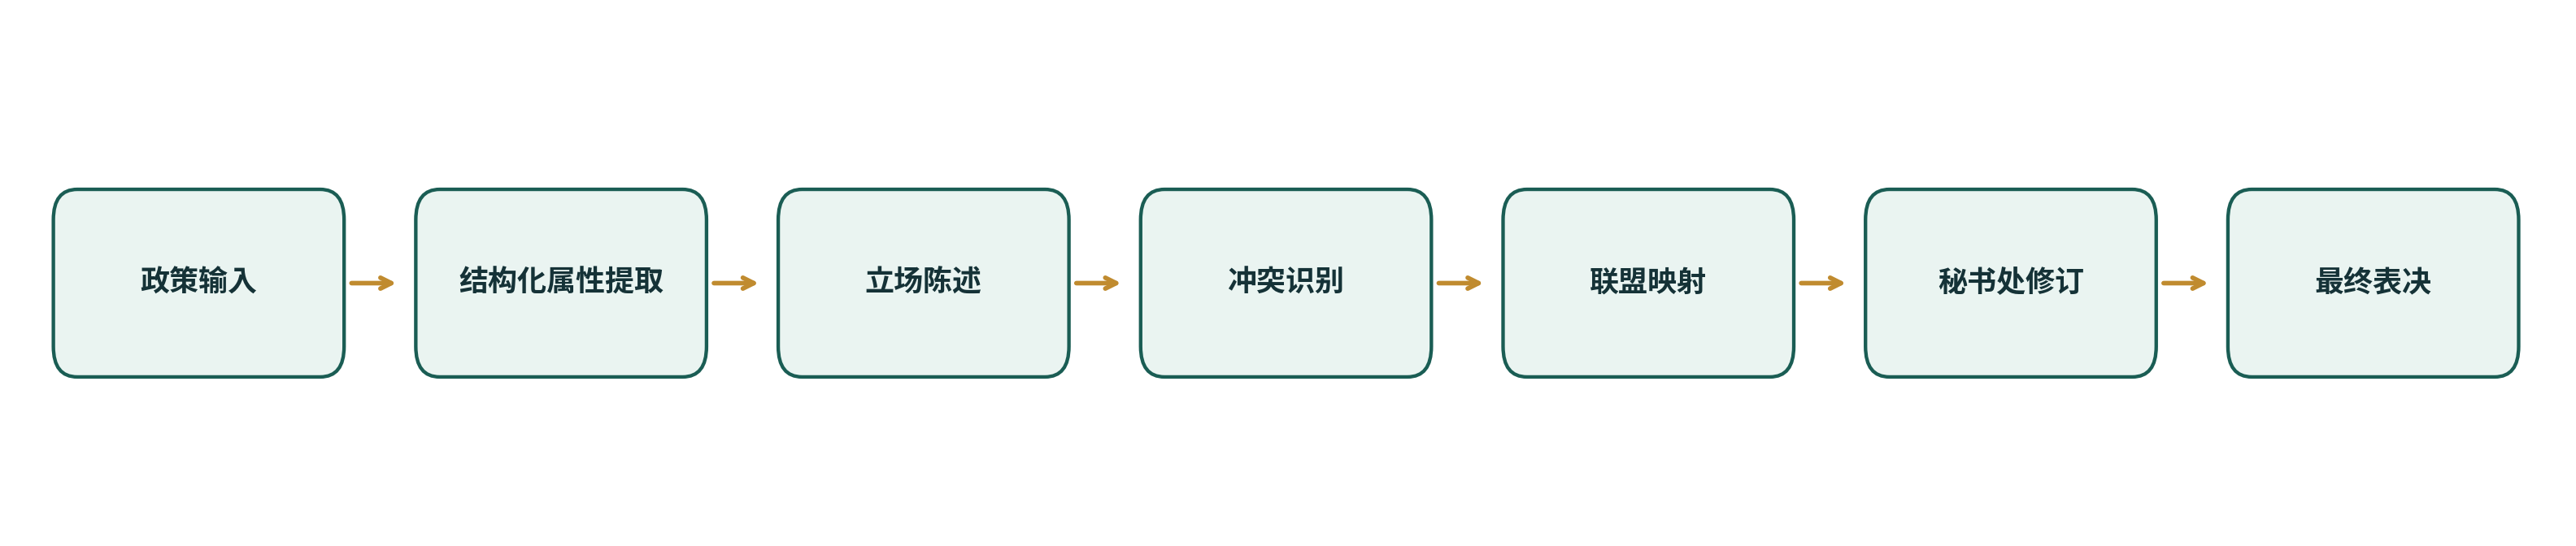
\includegraphics[width=0.98\textwidth]{figures/api_pipeline_overview.png}
  \caption{系统六阶段推演流程与结构化建模链路}
  \label{fig:pipeline}
\end{figure}

系统从政策输入到结果输出大致经历以下步骤：
\begin{enumerate}
  \item 读取政策文本，并结合关键词和显式属性生成结构化政策维度；
  \item 初始化角色对象或真实国家对象，载入偏好权重、基础倾向和约束条件；
  \item 由每个角色对当前政策做立场计算，得到分数、状态、支持点、担忧点和诉求；
  \item 汇总负向贡献，识别主要冲突来源；
  \item 根据共通诉求构建潜在联盟和摇摆方；
  \item 生成条件交换与秘书处修订方案；
  \item 在修订政策上重新进行最终表决，输出结果快照、Markdown 报告和 Web 可视化内容。
\end{enumerate}

\subsection{政策表示：从自然语言到结构化维度}
当前系统围绕 8 个核心维度建模：化石能源退出强度、碳边境约束强度、气候融资、技术转移、过渡期灵活性、CCS 支持、适应/损失补偿支持以及森林/LULUCF 支持。这一设计使系统能够把不同表述方式的政策文本放到统一的比较空间中。

例如，文本中出现 ``停止新建煤电''、``碳边境约束''、``适应融资''、``技术转移''、``森林保护'' 或 ``土地利用治理'' 等内容时，系统会自动抬升对应维度的强度值。随后，各角色不再面对一整段难以量化的自然语言，而是面对一组具有明确语义的结构化政策向量。

\subsection{形式化问题定义}
从方法上看，本文将系统建模为一个从政策文本到协商结果的映射问题。设政策文本经结构化处理后得到政策向量
\[
\mathbf{x}=(x_1,x_2,\dots,x_8), \qquad x_k \in \{0,1,2,3\},
\]
其中 8 个分量分别对应化石能源退出、碳边境约束、气候融资、技术转移、过渡期灵活性、CCS、适应/损失补偿以及森林/LULUCF 支持。设角色集合为
\[
\mathcal{A}=\{a_1,a_2,\dots,a_n\},
\]
每个角色 \(a_i\) 包含偏好权重向量 \(\mathbf{w}_i\)、基础倾向 \(b_i\)、优先诉求集合 \(P_i\)，以及在真实国家模式下额外存在的最小需求约束 \(R_i^{\min}\) 与最大容忍约束 \(R_i^{\max}\)。

在此基础上，系统需要完成三个层面的计算任务：
\begin{itemize}
  \item \textbf{角色评价}：给定 \(\mathbf{x}\) 后，计算各主体的分数、立场、支持点、担忧点和诉求；
  \item \textbf{协商修订}：根据初始反对压力和联盟结构，生成属性修订量 \(\Delta \mathbf{x}\)；
  \item \textbf{结果聚合}：将最终角色状态聚合为可行性、公平性、阻力强度和共识水平。
\end{itemize}
因此，系统的核心映射可以写为
\[
f:\ (\mathbf{x}, \mathcal{A}) \mapsto \bigl(\mathbf{y}, \Delta \mathbf{x}, s_{\mathrm{feas}}, s_{\mathrm{fair}}, s_{\mathrm{res}}, c \bigr),
\]
其中 \(\mathbf{y}\) 表示各角色最终立场集合，\(c\) 表示共识类别。

\subsection{评分函数与约束惩罚机制}
角色的原始得分由基础倾向与各维度加权贡献共同决定。对角色 \(a_i\) 而言，其原始得分定义为
\[
s_i^{\mathrm{raw}} = b_i + \sum_{k=1}^{8} w_{ik} x_k .
\]
这一定义与实现中的逐维线性累加完全一致，优点是解释路径清晰：任何一项政策属性的提高或降低，都会以可追溯的方式改变角色得分。

在真实国家样本模式下，系统进一步引入约束惩罚项。若某个维度低于最低需求，或者高于最大容忍值，则会对该角色施加惩罚：
\[
\mathrm{penalty}_i =
1.2 \sum_{k \in R_i^{\min}} \max(0, r_{ik}^{\min} - x_k)
+
1.2 \sum_{k \in R_i^{\max}} \max(0, x_k - r_{ik}^{\max}) .
\]
于是约束调整后的最终得分为
\[
s_i = s_i^{\mathrm{raw}} - \mathrm{penalty}_i .
\]
这种设计并不是简单地为现实国家附加若干 if-else，而是把收入水平、脆弱性、燃料出口暴露、目标类型与 NDC 条件性承诺转化为显式约束，从而把 ``现实边界'' 纳入协商模拟过程。

角色立场由得分阈值映射得到：
\[
\mathrm{status}(s_i)=
\begin{cases}
\text{支持}, & s_i \ge 4.0,\\
\text{有保留地支持}, & 1.2 \le s_i < 4.0,\\
\text{有保留地反对}, & -1.5 \le s_i < 1.2,\\
\text{强烈反对}, & s_i < -1.5.
\end{cases}
\]
这一阈值映射对应了系统中 ``支持--保留支持--保留反对--强烈反对'' 的四级分类框架。

\subsection{协商修订算法与聚合指标}
在形成初始立场后，系统不会直接输出结论，而是进一步计算反对压力并生成秘书处修订量。对每个政策维度 \(k\)，系统仅统计 ``有保留地反对'' 与 ``强烈反对'' 主体的压力；其中强烈反对记为 1.0，保留反对记为 0.6。若角色 \(a_i\) 希望强化某维度，则记为正向压力；若希望弱化该维度，则记为负向压力。由此定义维度压力
\[
p_k = \sum_{a_i \in \mathcal{O}} \alpha_i \cdot g_{ik},
\]
其中 \(\mathcal{O}\) 表示反对主体集合，\(\alpha_i \in \{1.0, 0.6\}\)，\(g_{ik}\in\{-1,0,1\}\) 表示该角色对维度 \(k\) 的修订方向。

最终修订量由阈值规则确定：
\[
\Delta x_k =
\begin{cases}
1, & p_k \ge 0.9,\\
-1, & p_k \le -0.9,\\
0, & \text{otherwise}.
\end{cases}
\]
随后，系统对修订后的 \(\mathbf{x}'=\mathbf{x}+\Delta \mathbf{x}\) 重新进行一次完整评价，并生成最终结果。

在结果聚合阶段，可行性、公平性和阻力强度分别定义为：
\[
\mathrm{Feasibility}=\frac{1}{3n}\sum_{i=1}^{n}\mathrm{score\_map}(\mathrm{status}_i)\times 100,
\]
\[
\mathrm{Fairness}=\frac{x'_{\mathrm{finance}}+x'_{\mathrm{tech}}+x'_{\mathrm{adapt}}+x'_{\mathrm{transition}}+x'_{\mathrm{lulucf}}}{15}\times 100,
\]
\[
\mathrm{Resistance}=100-\mathrm{Feasibility}+3 \cdot x'_{\mathrm{tariff}}.
\]
其中 \(\mathrm{score\_map}\) 将四类立场映射为 \(\{3,2,1,0\}\)。这些定义体现了本文的建模立场：可行性由总体支持分布决定，公平性主要由补偿、技术、适应、过渡和 LULUCF 支持决定，而阻力强度则在总体支持的基础上进一步考虑了贸易型约束带来的附加摩擦。

\subsection{关键算法伪代码}
为便于说明系统的计算链路，表~\ref{tab:algo-agent} 和表~\ref{tab:algo-revision} 给出了两个关键算法的伪代码表达。

\begin{table}[H]
\centering
\caption{角色评分与约束调整算法伪代码}
\label{tab:algo-agent}
\begin{tabularx}{\textwidth}{X}
\toprule
\texttt{Algorithm 1: EvaluateAgent(agent, policy\_attrs)} \\
\midrule
\texttt{1:\ \ score $\leftarrow$ base\_bias(agent)} \\
\texttt{2:\ \ for each feature k in FEATURE\_ORDER do} \\
\texttt{3:\ \ \ \ contribution[k] $\leftarrow$ weight(agent,k) * policy\_attrs[k]} \\
\texttt{4:\ \ \ \ score $\leftarrow$ score + contribution[k]} \\
\texttt{5:\ \ raw\_status $\leftarrow$ ThresholdMap(score)} \\
\texttt{6:\ \ Extract positive\_points and concern\_points from contribution} \\
\texttt{7:\ \ Build asks according to priority\_asks and current policy\_attrs} \\
\texttt{8:\ \ if constraint\_profile exists then} \\
\texttt{9:\ \ \ \ penalty $\leftarrow$ MinRequirementPenalty + MaxTolerancePenalty} \\
\texttt{10:\ \ \ score $\leftarrow$ score - penalty} \\
\texttt{11:\ \ \ status $\leftarrow$ ThresholdMap(score)} \\
\texttt{12:\ \ else status $\leftarrow$ raw\_status} \\
\texttt{13:\ \ statement $\leftarrow$ Narrator(role, status, positive\_points, concern\_points, asks)} \\
\texttt{14:\ \ return score, status, contribution, asks, statement} \\
\bottomrule
\end{tabularx}
\end{table}

\begin{table}[H]
\centering
\caption{压力驱动的修订生成算法伪代码}
\label{tab:algo-revision}
\begin{tabularx}{\textwidth}{X}
\toprule
\texttt{Algorithm 2: BuildRevision(initial\_vote, policy\_attrs)} \\
\midrule
\texttt{1:\ \ initialize pressure[k] $\leftarrow$ 0 for each feature k} \\
\texttt{2:\ \ for each role i in initial\_vote do} \\
\texttt{3:\ \ \ \ if status(i) not in \{conditional\_oppose, oppose\} then continue} \\
\texttt{4:\ \ \ \ intensity $\leftarrow$ 1.0 if oppose else 0.6} \\
\texttt{5:\ \ \ \ for each feature k in top priority asks of role i do} \\
\texttt{6:\ \ \ \ \ \ if weight(i,k) > 0 and policy\_attrs[k] < 3 then pressure[k] += intensity} \\
\texttt{7:\ \ \ \ \ \ else if weight(i,k) < 0 and policy\_attrs[k] > 0 then pressure[k] -= intensity} \\
\texttt{8:\ \ for each feature k do} \\
\texttt{9:\ \ \ \ if pressure[k] $\ge$ 0.9 then adjustment[k] $\leftarrow$ +1} \\
\texttt{10:\ \ \ else if pressure[k] $\le$ -0.9 then adjustment[k] $\leftarrow$ -1} \\
\texttt{11:\ \ \ else adjustment[k] $\leftarrow$ 0} \\
\texttt{12:\ \ return adjustment and revised policy vector} \\
\bottomrule
\end{tabularx}
\end{table}

\subsection{抽象角色模式}
抽象角色模式包含 7 类主体：发达国家联盟、大型新兴经济体、最不发达国家集团、小岛屿与高脆弱国家联盟、化石能源出口国集团、清洁技术与低碳产业联盟、多边开发金融机构。每个角色都包含以下信息：
\begin{itemize}
  \item 身份和阵营说明；
  \item 设计依据和证据基础；
  \item 优先诉求；
  \item 不同政策维度上的偏好权重；
  \item 基础倾向值。
\end{itemize}

图~\ref{fig:weight-heatmap} 给出了抽象角色在不同政策维度上的偏好权重矩阵。这张图的重要性在于，它能够直接说明为什么不同角色会对同一政策产生不同反应：例如，发达国家联盟对化石退出和碳边境约束给出较高正权重，而化石能源出口国集团对化石退出和碳边境约束则给出显著负权重。

\begin{figure}[H]
  \centering
  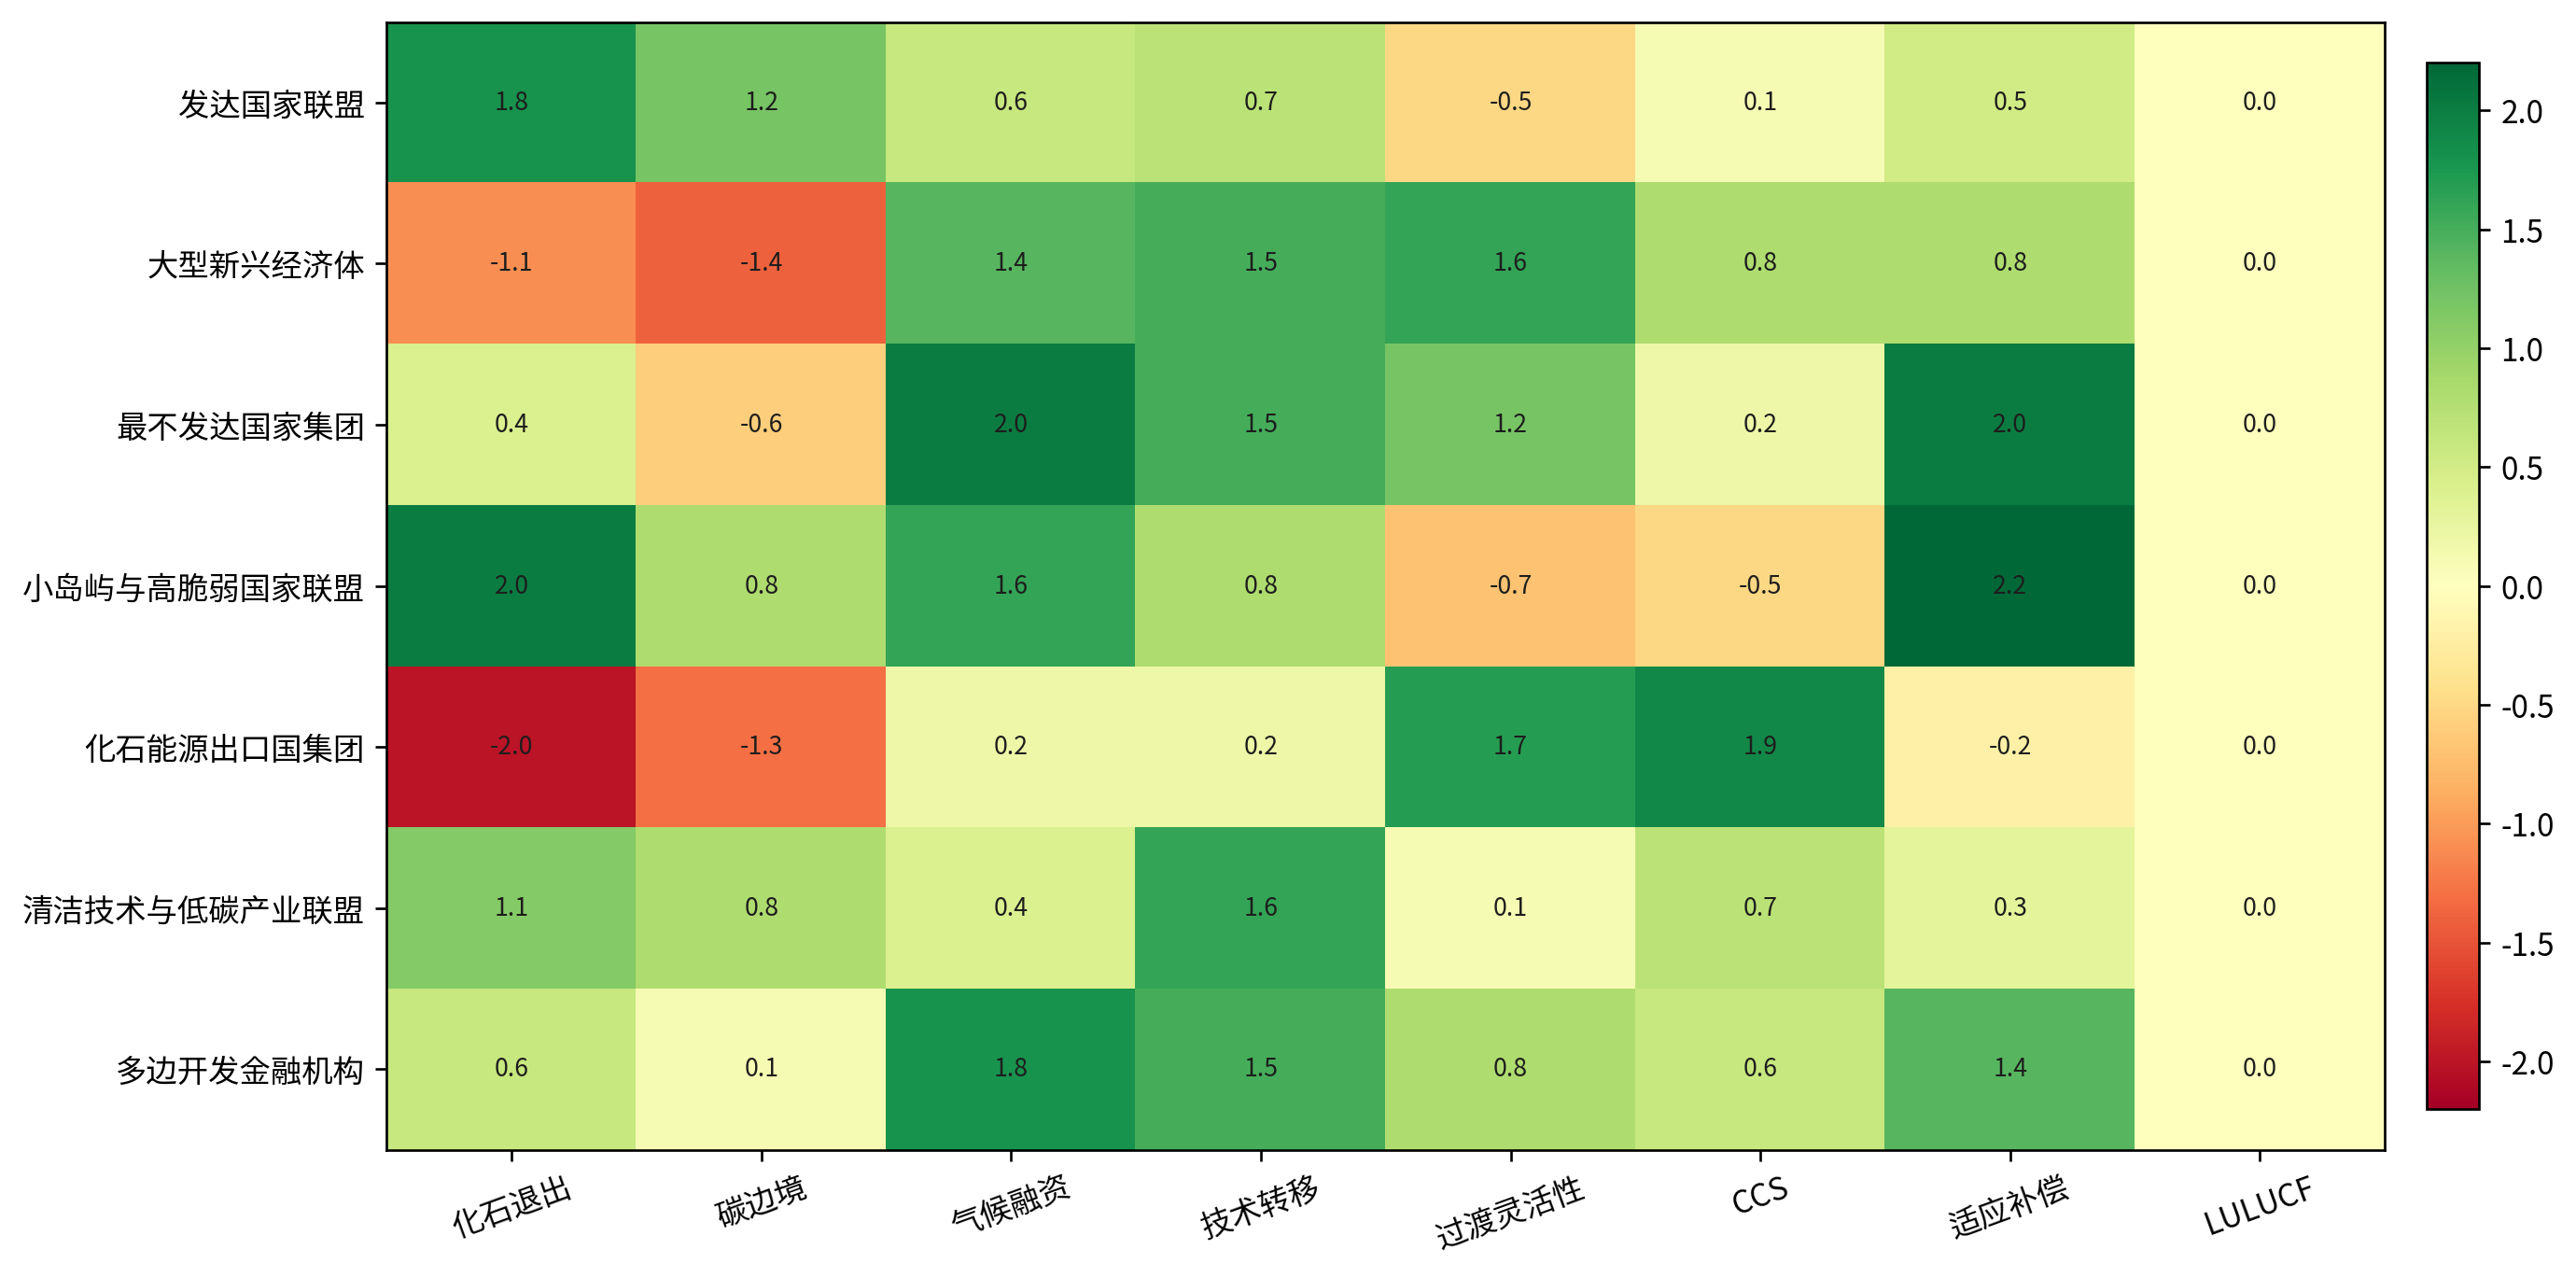
\includegraphics[width=0.92\textwidth]{figures/api_role_weight_heatmap.png}
  \caption{抽象角色配置中的政策偏好权重矩阵}
  \label{fig:weight-heatmap}
\end{figure}

\subsection{真实国家样本模式}
为了让系统从 ``典型角色'' 走向 ``有真实来源约束的样本国家''，本文进一步构建了真实国家样本模式。当前样本包括德国、美国、中国、巴西、印度、印度尼西亚、沙特阿拉伯、斐济和孟加拉国。

在该模式下，角色不再完全由人工写死，而是综合以下信息生成：
\begin{itemize}
  \item 世界银行开放数据中的 GDP、人均收入、可再生能源占比和燃料出口占比；
  \item ND-GAIN 的脆弱性与准备度指标；
  \item UNFCCC NDC Registry 与 Climate Watch 中的结构化 NDC 摘要；
  \item 是否存在条件性融资/技术需求；
  \item 是否涉及森林、碳汇和土地利用治理。
\end{itemize}

系统在此基础上进一步生成两类硬约束：\texttt{min\_requirements} 与 \texttt{max\_tolerances}。前者表示最低需要满足的支持项，例如适应资金或技术转移；后者表示最大可容忍的政策强度，例如过强的化石退出或碳边境约束。一旦政策触发这些约束，角色立场就会被系统显式下调，并记录触发原因。

\subsection{六阶段协商流程}
系统的协商流程固定为六阶段：立场陈述、冲突识别、联盟与分裂、条件交换、秘书处修订、最终表决。它并不是一个每个 agent 独立线程自由对话的自治多智能体系统，而是一个 \textbf{规则驱动的多角色协商引擎}。这种设计的优点是：
\begin{itemize}
  \item 输出稳定，可重复运行；
  \item 决策路径清晰，便于报告写作；
  \item 便于展示与解释；
  \item 能够在不牺牲可解释性的前提下接入 DeepSeek V4 Pro 做叙事增强。
\end{itemize}

\subsection{DeepSeek V4 Pro 叙事增强层}
系统中的 LLM 适配层采用 OpenAI-compatible 接口封装。为保证实验可重复，当前实验环境采用如下配置：
\begin{itemize}
  \item Base URL：\texttt{https://opencode.ai/zen/go/v1}
  \item API Path：\texttt{chat/completions}
  \item Model：\texttt{deepseek-v4-pro}
\end{itemize}

在我们的实现中，DeepSeek V4 Pro 并不直接决定政策分数与投票结果，这些量化结果仍由规则引擎计算；它接收 ``角色背景--当前态度--支持点--担忧点--诉求'' 这一结构化状态，并将其组织为更自然、接近真实谈判语境的中文发言。也正因为采用了这种解耦设计，我们才能同时保证量化指标的可复现性和展示语言的可读性。

\subsection{Web 展示、历史回放与结果导出}
除核心推演引擎外，我们还实现了基于 Streamlit 的展示层，用于支撑课堂演示和结果复查。该展示层至少覆盖了四类功能：
\begin{itemize}
  \item \textbf{政策输入与模式切换}：支持输入政策文本，并在抽象角色模式与真实国家样本模式之间切换；
  \item \textbf{单次推演与批量情景实验}：既可以运行单条政策，也可以对预设情景做成组比较；
  \item \textbf{历史记录与结果回放}：系统会将单次运行结果保存为本地快照，便于在课堂上复现先前实验，而不是每次都从零开始演示；
  \item \textbf{报告导出与图表生成}：系统能够输出结构化 JSON、Markdown 报告以及后续用于技术报告的统计图表。
\end{itemize}
这一部分虽然不直接改变谈判分数，却直接决定了系统是否便于展示、是否支持复现、是否能够沉淀为正式提交材料。因此，从完整交付的角度看，Web 展示层、历史记录与结果导出功能也是系统的重要组成部分。

\subsection{关键代码模块与项目组织}
为了更完整地交代系统的实现内容，我们将其按 ``核心引擎--叙事接口--展示层--数据层--实验层'' 五个部分来理解：
\begin{itemize}
  \item \textbf{核心引擎}：\texttt{prototype\_v1/climate\_policy\_engine.py} 是整个系统的计算中枢，负责政策属性抽取、角色评价、冲突识别、联盟构建、秘书处修订与最终报告生成；
  \item \textbf{叙事接口}：\texttt{prototype\_v1/llm\_adapter.py} 封装模板叙事器与 OpenAI-compatible 叙事器，使系统能够在无 API 和有 API 的两种条件下运行；
  \item \textbf{展示层}：\texttt{prototype\_v1/streamlit\_app.py} 提供课堂演示所需的人机界面，\texttt{run\_demo.py} 与 \texttt{run\_llm\_demo.py} 则用于命令行演示与快速验证；
  \item \textbf{数据层}：\texttt{data/agents.json}、\texttt{data/real\_world\_entities.json}、\texttt{data/real\_policy\_profiles.json} 与 \texttt{data/source\_catalog.json} 分别承担抽象角色配置、国家客观指标、NDC 摘要信息和数据来源管理；
  \item \textbf{实验层}：\texttt{results/} 用于保存单次运行结果和历史快照，\texttt{submission\_original/scripts/} 下的脚本负责正式实验、图表生成与提交材料整理。
\end{itemize}
采用这样的组织方式有两个直接好处：一方面，系统结构足够清晰，便于我们在报告中解释每一部分各自承担的任务；另一方面，也为后续继续扩展为更真实的多 agent 版本保留了清晰的升级接口。

\section{实验设计}

\subsection{实验原则}
本文仅引用本轮实验中实际运行得到的结果，不使用历史快照替代当前实验结论。为兼顾覆盖度、真实性和分析深度，我们选取了一组核心实验集，包括四个单次实验、两组情景实验以及一组方法层面的模块对比实验。

\subsection{实验环境与真实性约束}
本报告写入的结果均由脚本 \texttt{submission\_original/scripts/run\_api\_core\_experiments.py} 和 \texttt{submission\_original/scripts/run\_api\_method\_ablation.py} 实际运行得到，并分别汇总到 \texttt{api\_core\_experiment\_summary.json} 与 \texttt{api\_method\_ablation\_summary.json}。我们在这里说明两点：
\begin{itemize}
  \item \textbf{真实性约束}：正文中的数值、共识水平、约束触发次数和角色发言样例均来自实际 API 运行产物，而非手工编造；
  \item \textbf{职责分工}：规则引擎负责可行性、公平性、阻力强度和约束触发的计算，DeepSeek V4 Pro 负责将结构化状态转写为自然语言谈判表达。
\end{itemize}

\subsection{实验矩阵}
表~\ref{tab:exp-matrix} 给出了本次写入报告的核心实验矩阵。

\begin{table}[H]
\centering
\caption{本报告使用的 API 核心实验矩阵}
\label{tab:exp-matrix}
\begin{tabularx}{\textwidth}{>{\raggedright\arraybackslash}p{3cm} >{\raggedright\arraybackslash}p{2.2cm} >{\raggedright\arraybackslash}X}
\toprule
实验编号 & 主体模式 & 实验目的 \\
\midrule
E1 & 抽象角色 & 运行高冲突煤电退出 + 碳边境约束政策，观察强冲突下的阻力结构 \\
E2 & 抽象角色 & 运行平衡型综合政策，观察在补偿和过渡安排存在时是否形成较强共识 \\
E3 & 真实国家样本 & 在真实国家约束下运行平衡型综合政策，观察现实摩擦对可行性的影响 \\
E4 & 真实国家样本 & 运行森林治理与公平融资政策，测试 LULUCF 与公平补偿对结果的影响 \\
E5 & 抽象角色情景实验 & 在 4 个预设情景中比较可行性、公平性与阻力强度 \\
E6 & 真实国家情景实验 & 在 4 个预设情景中比较可行性、公平性、阻力强度与现实约束触发频次 \\
E7 & 方法模块对比实验 & 比较显式属性、文本自动识别、秘书处修订和现实约束建模对结果的影响 \\
\bottomrule
\end{tabularx}
\end{table}

\subsection{实验政策文本}
本次实验中使用的代表性政策文本包括：
\begin{itemize}
  \item \textbf{高冲突样例政策}：强调 2030 年前停止新建无减排措施煤电并提高碳边境约束；
  \item \textbf{平衡型综合政策}：同时强调煤电限制、适应融资、技术转移、森林/LULUCF 和分阶段过渡安排；
  \item \textbf{森林治理与公平融资政策}：突出森林保护、碳汇治理、损失损害支持、技术转移和更长过渡期。
\end{itemize}

\subsection{评价指标}
本报告主要使用以下指标：
\begin{itemize}
  \item \textbf{可行性}：以最终角色状态映射而来的总体支持程度；
  \item \textbf{公平性}：基于融资、技术转移、适应支持、过渡安排和 LULUCF 支持的综合度量；
  \item \textbf{阻力强度}：基于总体支持度与约束压力计算出的推进阻力；
  \item \textbf{共识水平}：分为较强共识、脆弱共识、有限妥协和分歧明显；
  \item \textbf{约束触发次数}：仅在真实国家样本的情景实验中记录，用于描述现实边界的刚性程度。
\end{itemize}

\section{实验结果与分析}

\subsection{四组核心单次实验结果}
图~\ref{fig:single-metrics} 展示了四组核心单次实验的结果对比，表~\ref{tab:single-result} 则给出具体数值。

\begin{figure}[H]
  \centering
  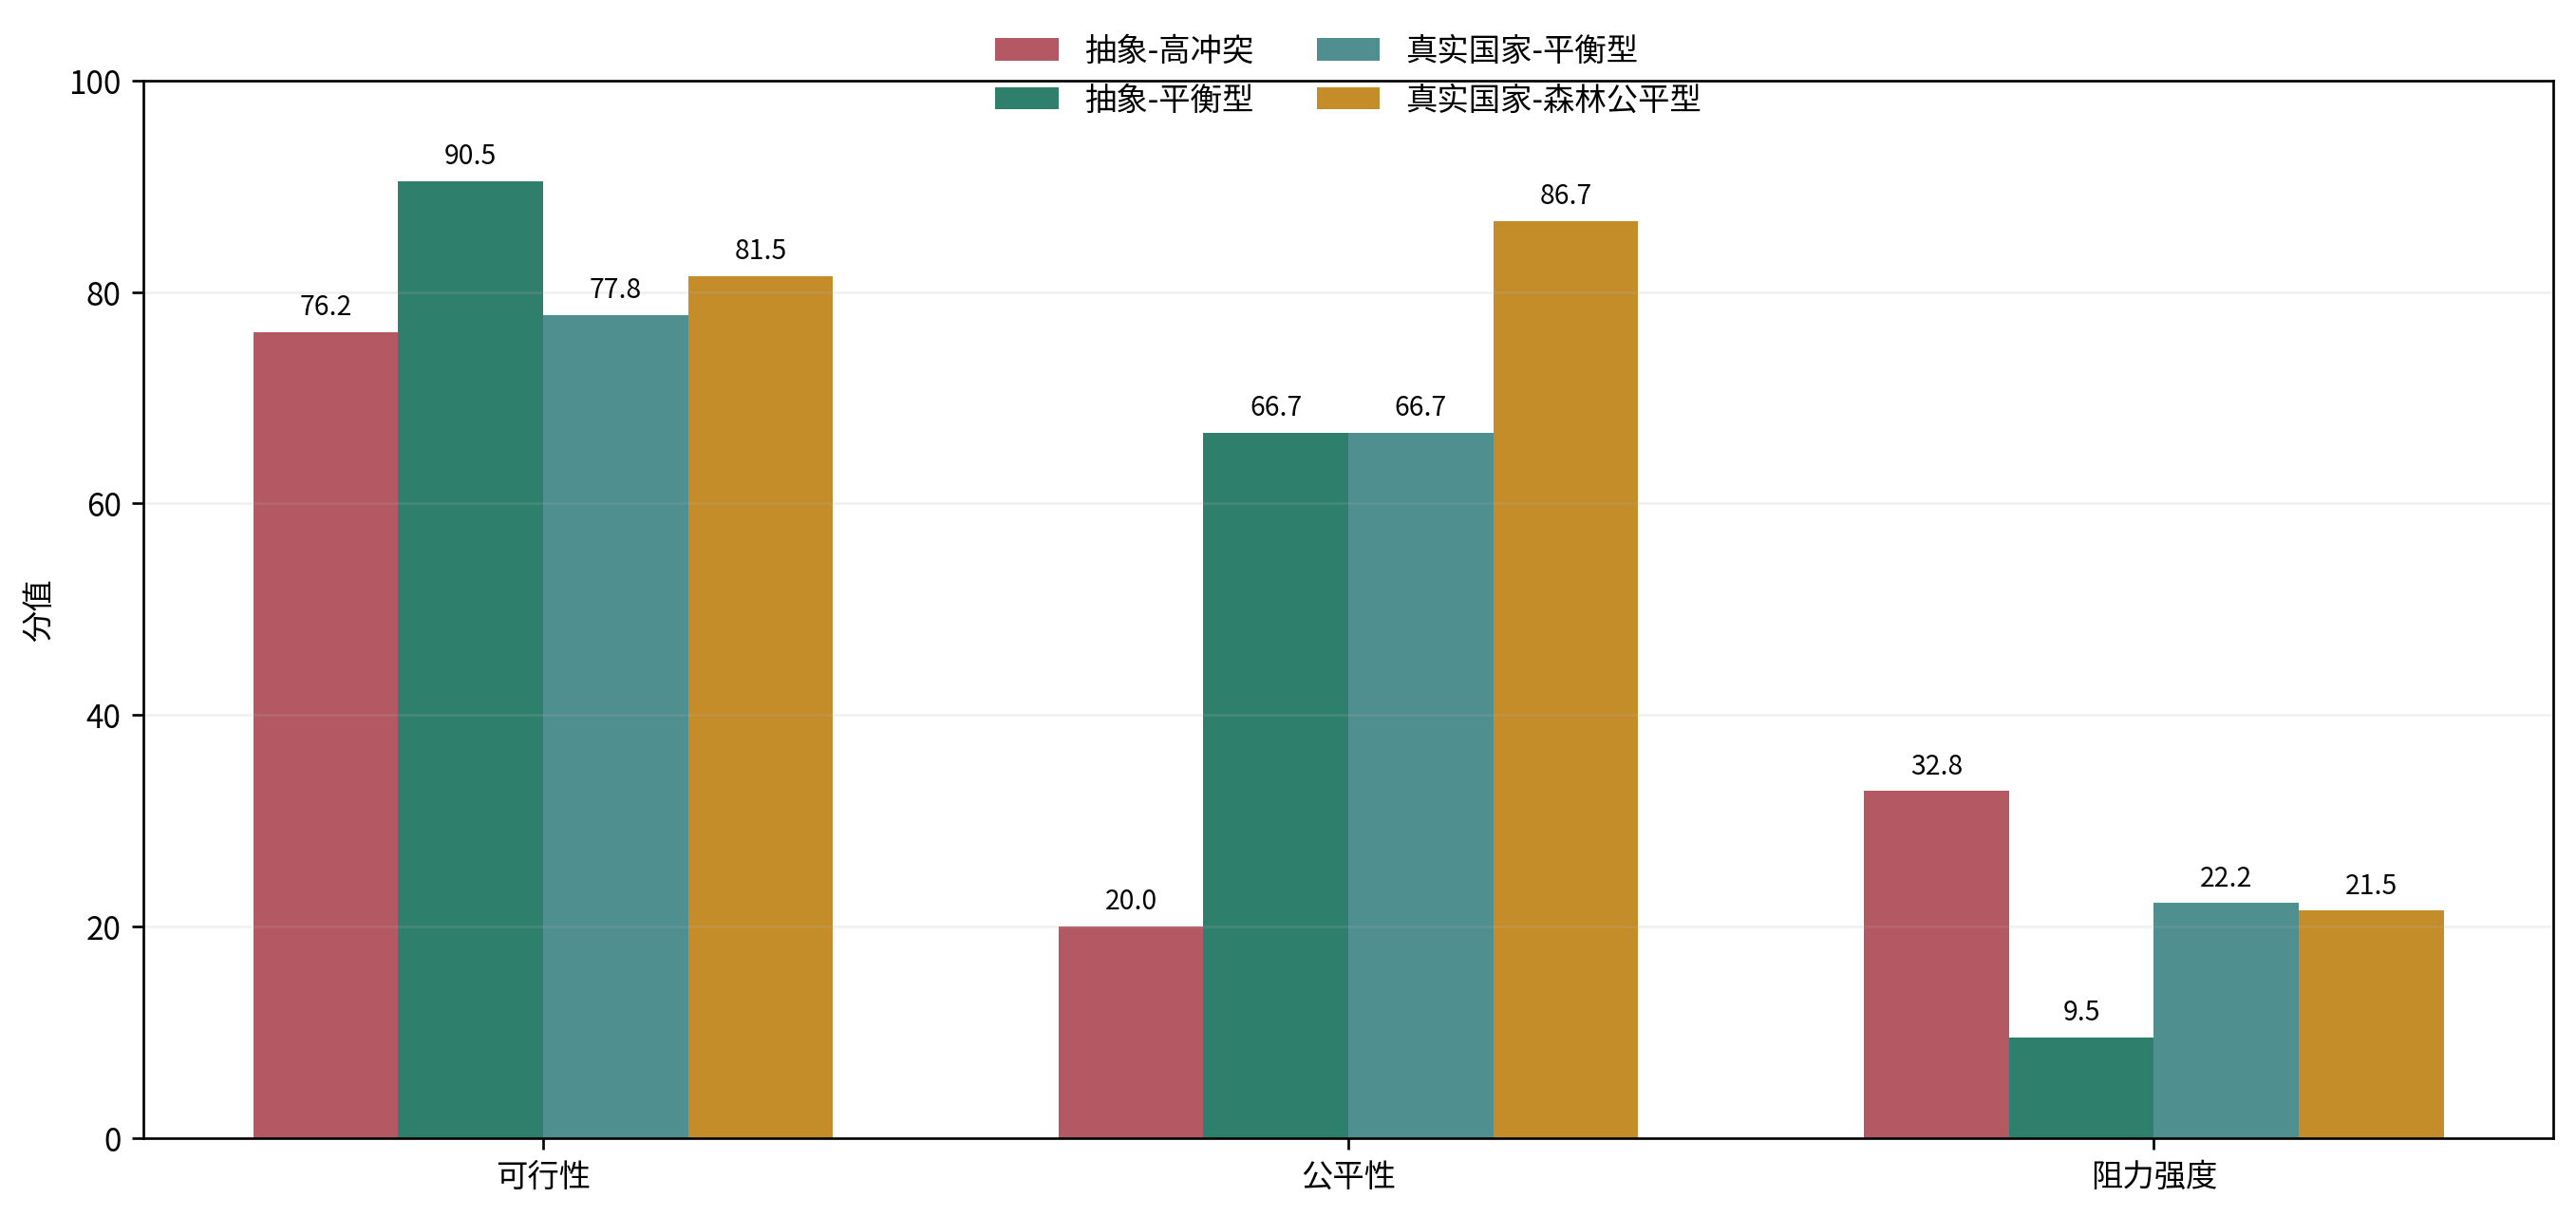
\includegraphics[width=0.95\textwidth]{figures/api_single_metrics_comparison.png}
  \caption{四组 API 单次实验的核心指标对比}
  \label{fig:single-metrics}
\end{figure}

\begin{table}[H]
\centering
\caption{四组 API 单次实验结果}
\label{tab:single-result}
\begin{tabular}{lcccc}
\toprule
实验 & 共识水平 & 可行性 & 公平性 & 阻力强度 \\
\midrule
E1 抽象-高冲突 & 有限妥协 & 76.2 & 20.0 & 32.8 \\
E2 抽象-平衡型 & 较强共识 & 90.5 & 66.7 & 9.5 \\
E3 真实国家-平衡型 & 较强共识 & 77.8 & 66.7 & 22.2 \\
E4 真实国家-森林公平型 & 较强共识 & 81.5 & 86.7 & 21.5 \\
\bottomrule
\end{tabular}
\end{table}

这些结果可以支撑三个直接结论：
\begin{enumerate}
  \item \textbf{高冲突政策确实会显著恶化结果}。在 E1 中，公平性只有 20.0，阻力强度达到 32.8，说明当政策只有退出和约束、没有配套支持时，系统迅速识别出难以调和的冲突。
  \item \textbf{平衡型政策在抽象角色模式下更容易形成稳定共识}。E2 的可行性提升到 90.5，阻力强度降到 9.5，说明加入融资、技术转移、适应支持和过渡安排后，原本的主要反对方会明显缓和。
  \item \textbf{真实国家约束会拉低同一政策的表面可行性}。E3 相比 E2 可行性下降到 77.8，阻力强度升到 22.2，说明现实世界中的收入水平、燃料出口暴露、NDC 类型和条件性承诺，确实会让系统更保守。
\end{enumerate}

同时，E4 显示：当政策显式突出森林治理、碳汇与公平融资时，公平性可上升到 86.7，并在真实国家样本模式下保持 81.5 的可行性。这说明 \textbf{森林/LULUCF 并不是边角议题，而是提升森林型新兴经济体与高脆弱国家接受度的重要抓手。}

\subsection{抽象角色情景实验}
图~\ref{fig:abstract-batch} 展示了抽象角色模式下四个 API 情景实验的对比结果。

\begin{figure}[H]
  \centering
  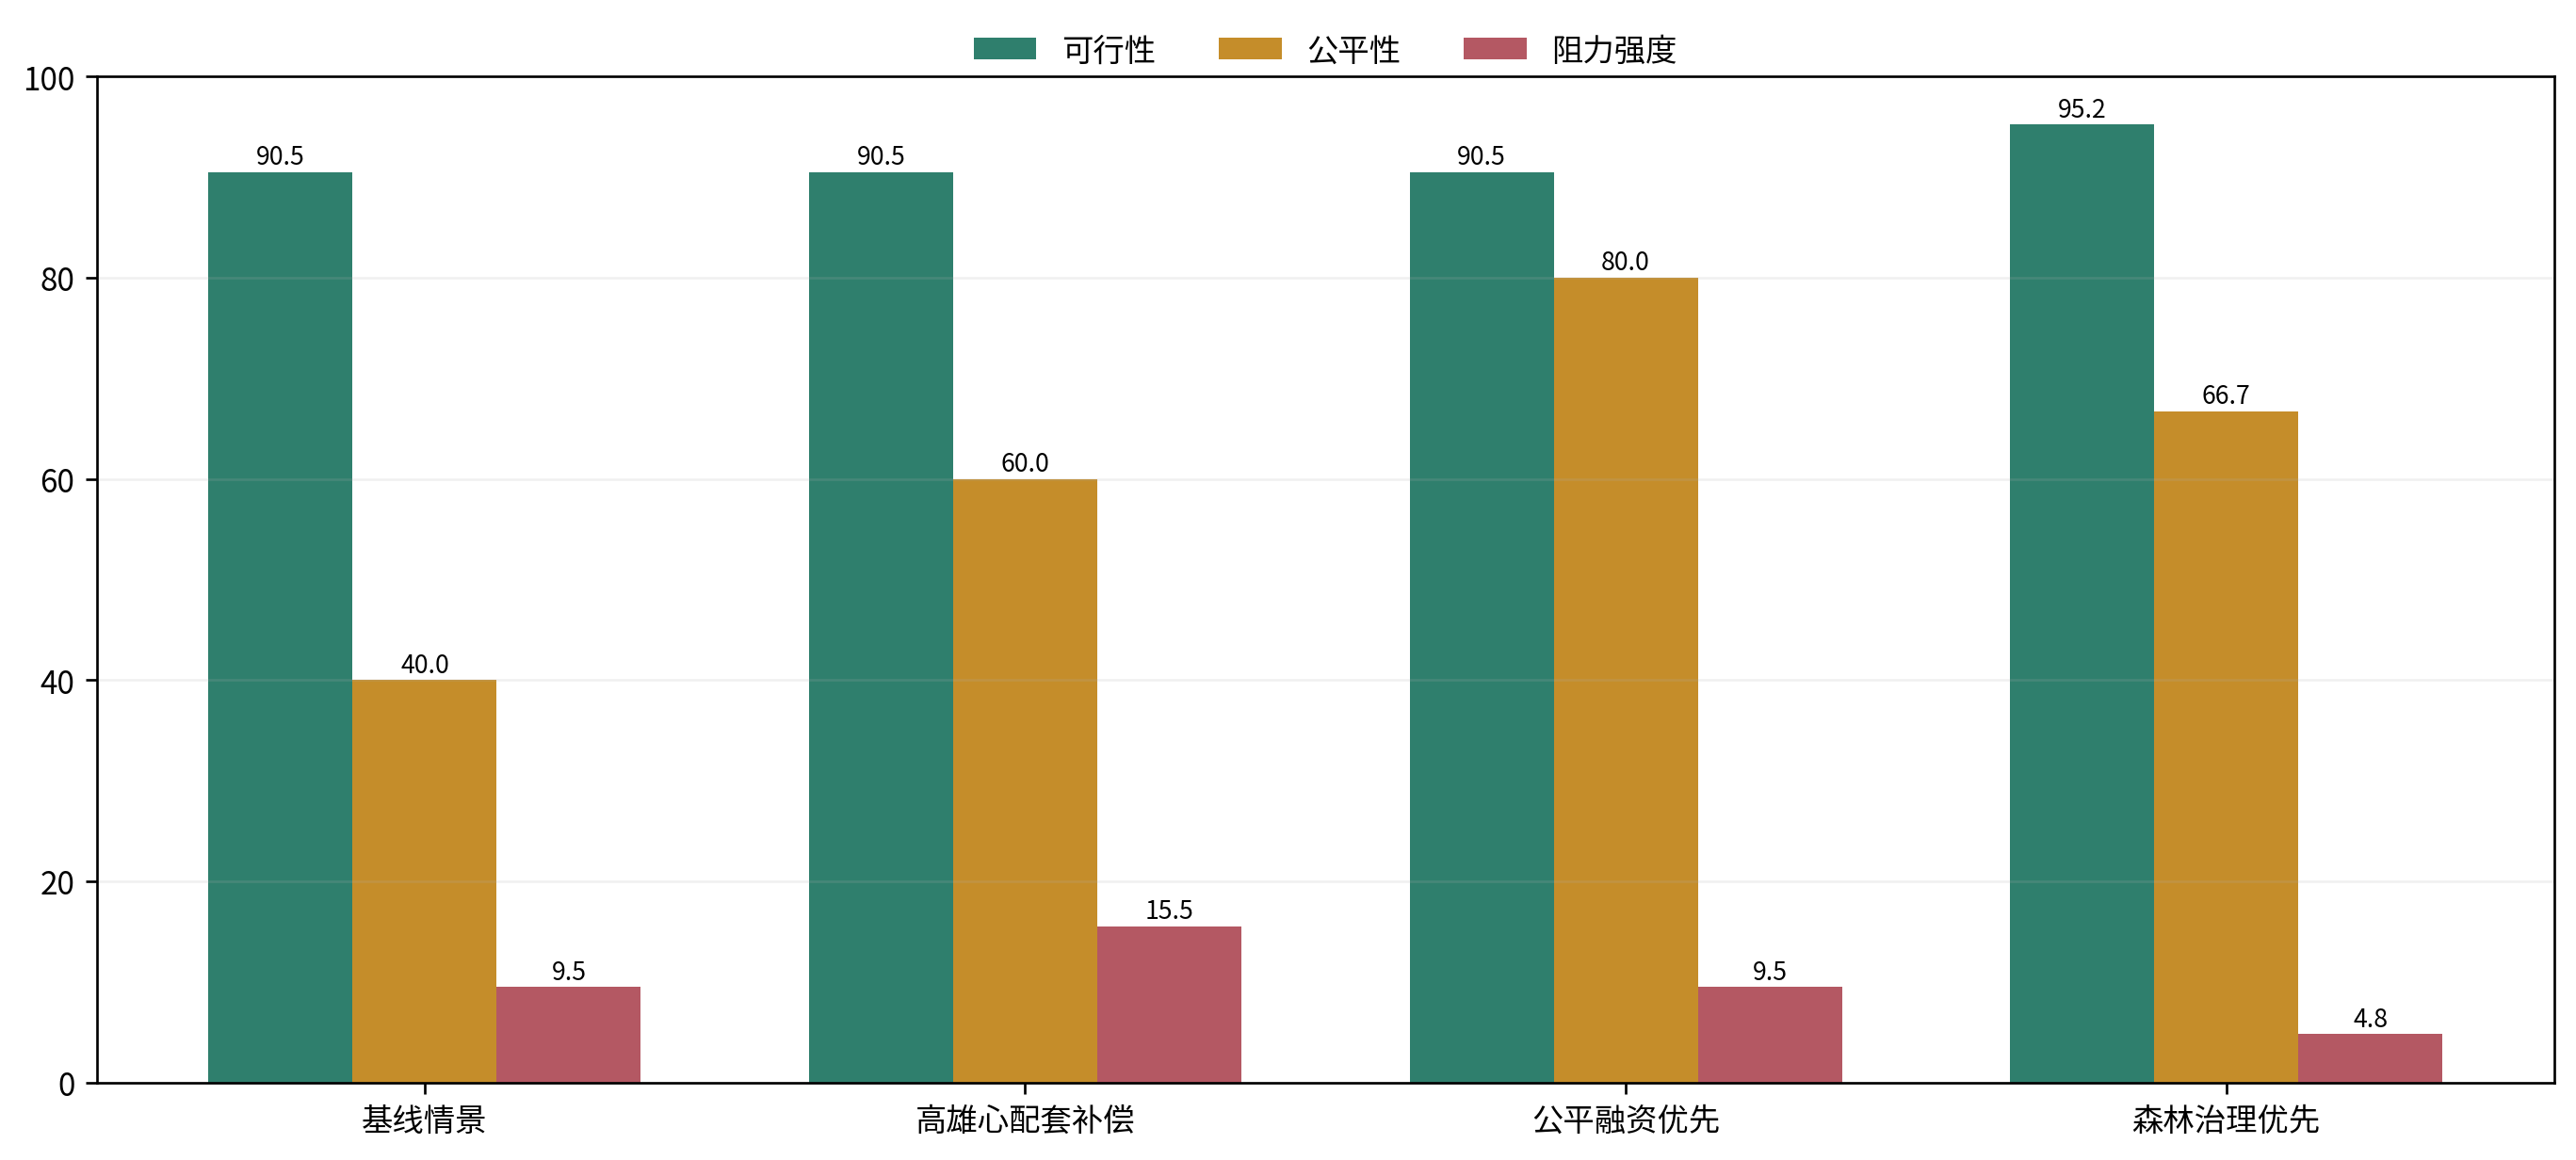
\includegraphics[width=0.96\textwidth]{figures/api_abstract_batch_compare.png}
  \caption{抽象角色模式下的 API 情景实验对比}
  \label{fig:abstract-batch}
\end{figure}

\begin{table}[H]
\centering
\caption{抽象角色模式下的 API 情景实验结果}
\label{tab:abstract-batch}
\begin{tabular}{lcccc}
\toprule
情景 & 共识水平 & 可行性 & 公平性 & 阻力强度 \\
\midrule
基线情景 & 较强共识 & 90.5 & 40.0 & 9.5 \\
高雄心配套补偿 & 较强共识 & 90.5 & 60.0 & 15.5 \\
公平融资优先 & 较强共识 & 90.5 & 80.0 & 9.5 \\
森林治理优先 & 较强共识 & 95.2 & 66.7 & 4.8 \\
\bottomrule
\end{tabular}
\end{table}

从结果可以看出：
\begin{itemize}
  \item ``森林治理优先'' 情景的可行性最高，为 95.2，阻力最低，仅为 4.8；
  \item ``公平融资优先'' 情景的公平性最高，为 80.0；
  \item ``高雄心配套补偿'' 虽然保持了 90.5 的可行性，但阻力提升到 15.5，说明抽象角色模式下，即使加入配套补偿，高雄心减排仍然带来一定摩擦。
\end{itemize}

这说明在抽象角色视角下，\textbf{森林/LULUCF 和公平融资安排都能有效减轻主要分歧，而一味强化减排目标即便附带补偿，也不一定是最优路径。}
同时，实验摘要显示抽象角色模式中对情景变化最敏感的主体是 \textbf{发达国家联盟}。这意味着在当前角色构型中，发达国家联盟往往扮演 ``规则强度调节器'' 的角色：当文本更强调公平融资和森林治理时，它能够保持支持；当文本进一步提高减排强度但责任分担写得不够清晰时，其保留意见也会更早暴露出来。

\subsection{真实国家情景实验}
真实国家模式的情景实验结果如图~\ref{fig:real-batch} 所示。

\begin{figure}[H]
  \centering
  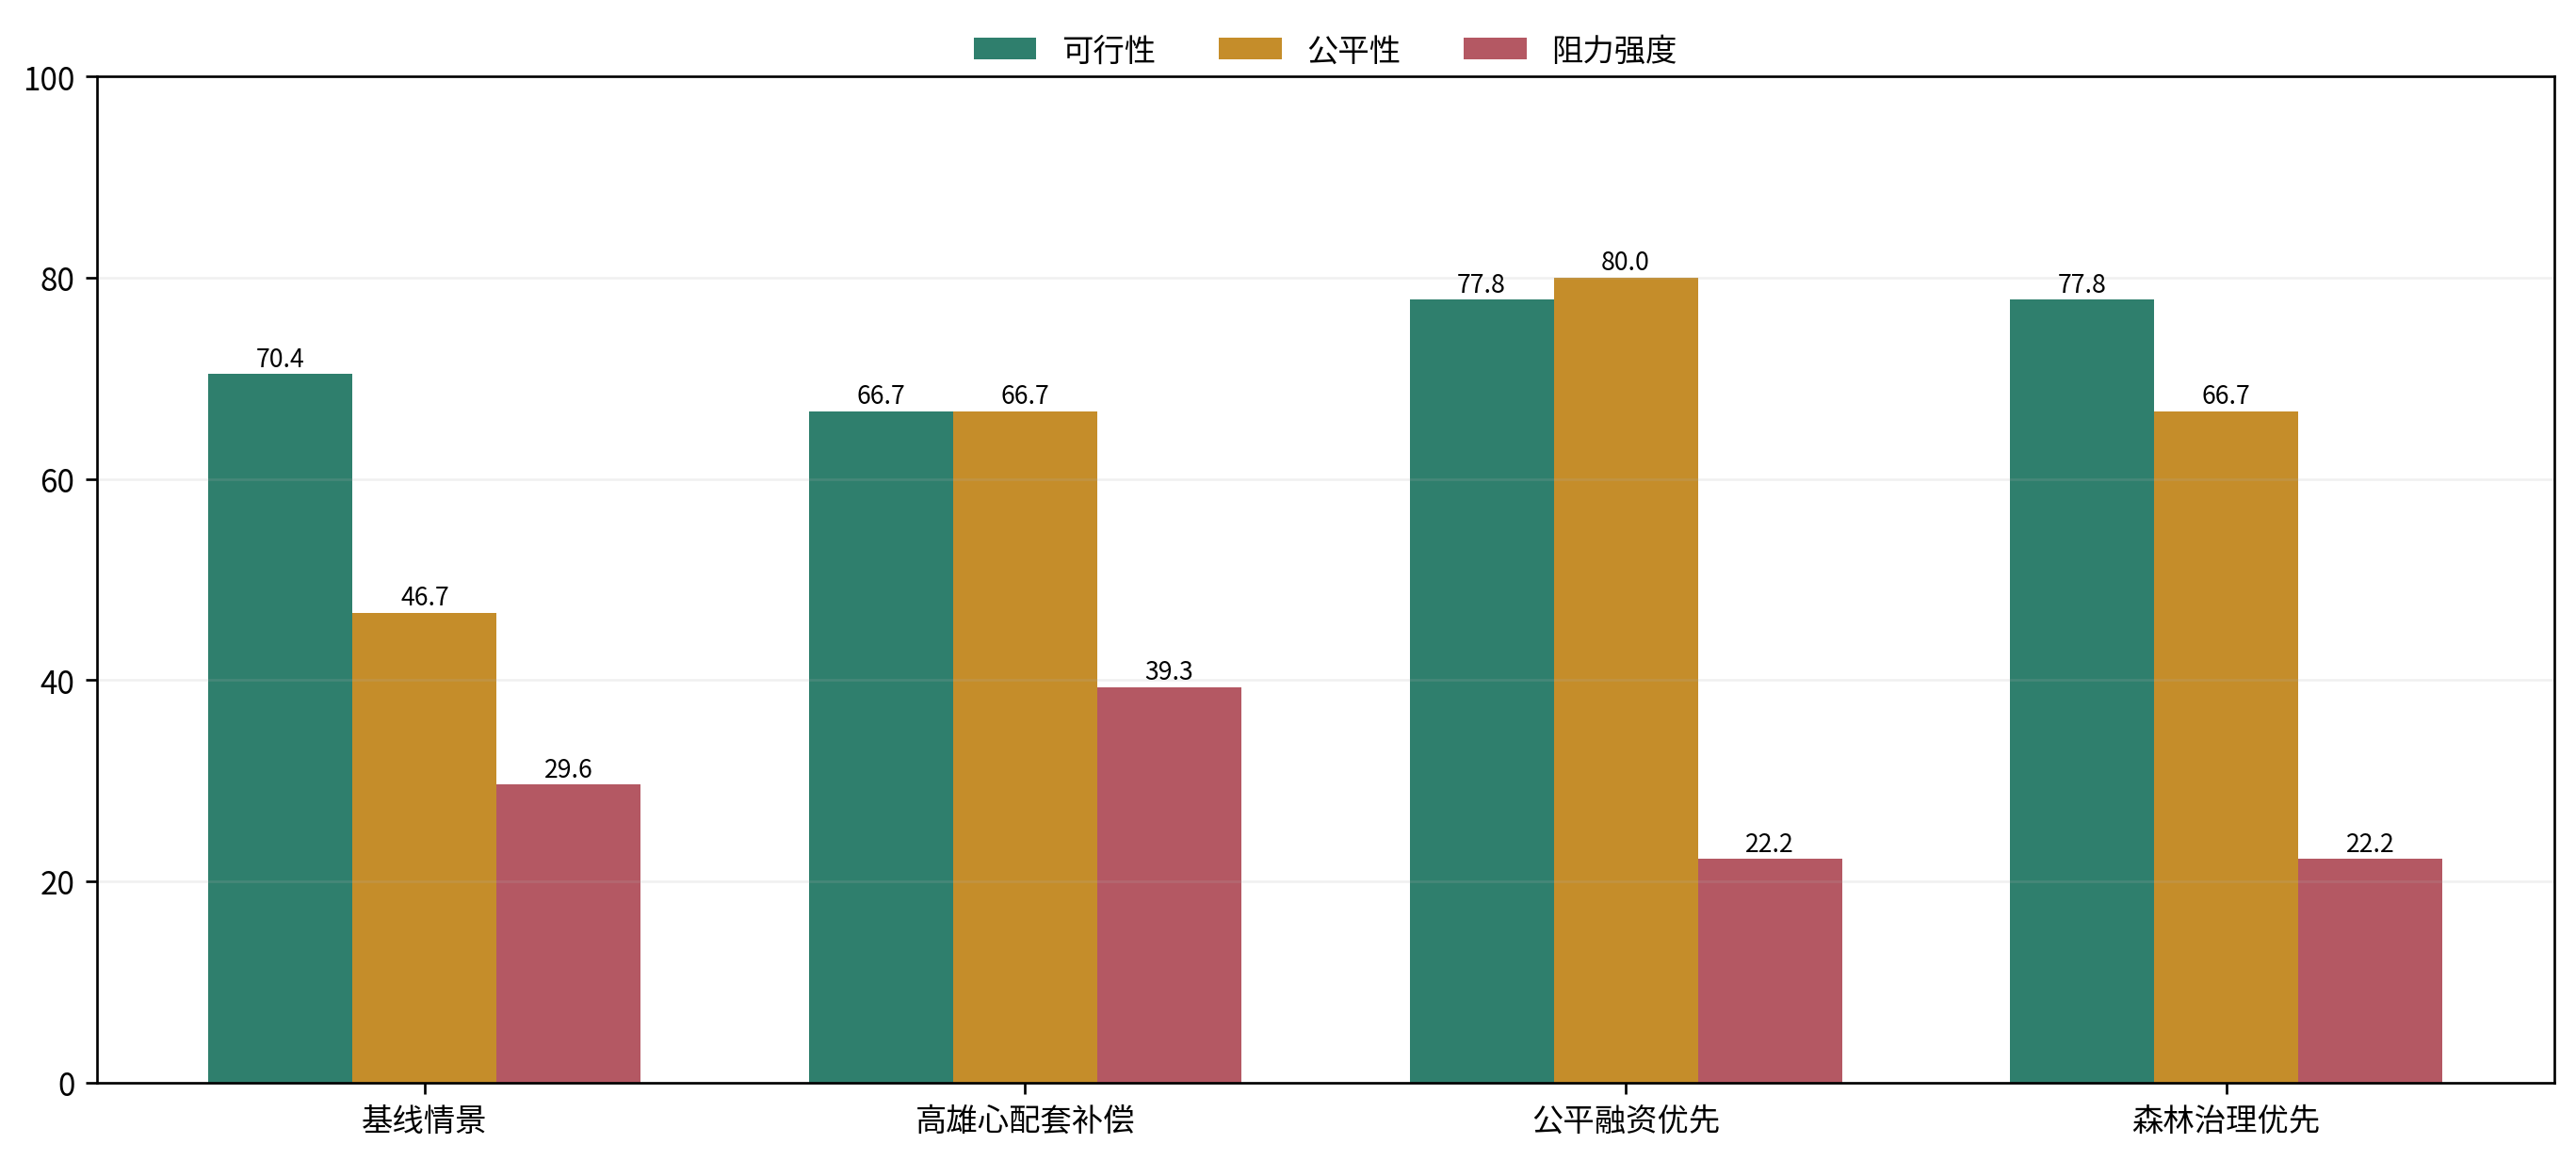
\includegraphics[width=0.96\textwidth]{figures/api_real_batch_compare.png}
  \caption{真实国家样本模式下的 API 情景实验对比}
  \label{fig:real-batch}
\end{figure}

\begin{table}[H]
\centering
\caption{真实国家样本模式下的 API 情景实验结果}
\label{tab:real-batch}
\begin{tabular}{lccccc}
\toprule
情景 & 共识水平 & 可行性 & 公平性 & 阻力强度 & 约束触发次数 \\
\midrule
基线情景 & 脆弱共识 & 70.4 & 46.7 & 29.6 & 5 \\
高雄心配套补偿 & 有限妥协 & 66.7 & 66.7 & 39.3 & 10 \\
公平融资优先 & 较强共识 & 77.8 & 80.0 & 22.2 & 2 \\
森林治理优先 & 较强共识 & 77.8 & 66.7 & 22.2 & 2 \\
\bottomrule
\end{tabular}
\end{table}

与抽象角色模式相比，真实国家样本模式呈现出更强的现实摩擦：
\begin{itemize}
  \item 基线情景只有 70.4 的可行性，且出现 5 次现实约束触发；
  \item ``高雄心配套补偿'' 虽然公平性提升到 66.7，但可行性下降到 66.7、阻力上升到 39.3，同时触发 10 次现实约束；
  \item ``公平融资优先'' 成为真实国家模式中综合表现最好的情景，可行性 77.8、公平性 80.0、阻力 22.2；
  \item ``森林治理优先'' 与 ``公平融资优先'' 的可行性相同，但公平性稍低，说明森林议题的重要性依然需要借助融资和适应安排才能被充分转化为共识。
\end{itemize}

这组结果说明：\textbf{在更贴近现实的国家模式下，公平融资优先比单纯高雄心配套补偿更能形成可持续共识。}
实验摘要还指出，真实国家模式中对情景变化最敏感的主体是 \textbf{沙特阿拉伯}。这与其高资源出口暴露、对退出时程和碳边境约束极为敏感的角色设定一致，也说明真实国家模式确实捕捉到了 ``化石能源出口国在高强度转型方案中更容易转为关键阻力点'' 这一现实特征。

\subsection{现实约束触发分析}
图~\ref{fig:constraint} 展示了真实国家情景实验中的现实约束触发频次。

\begin{figure}[H]
  \centering
  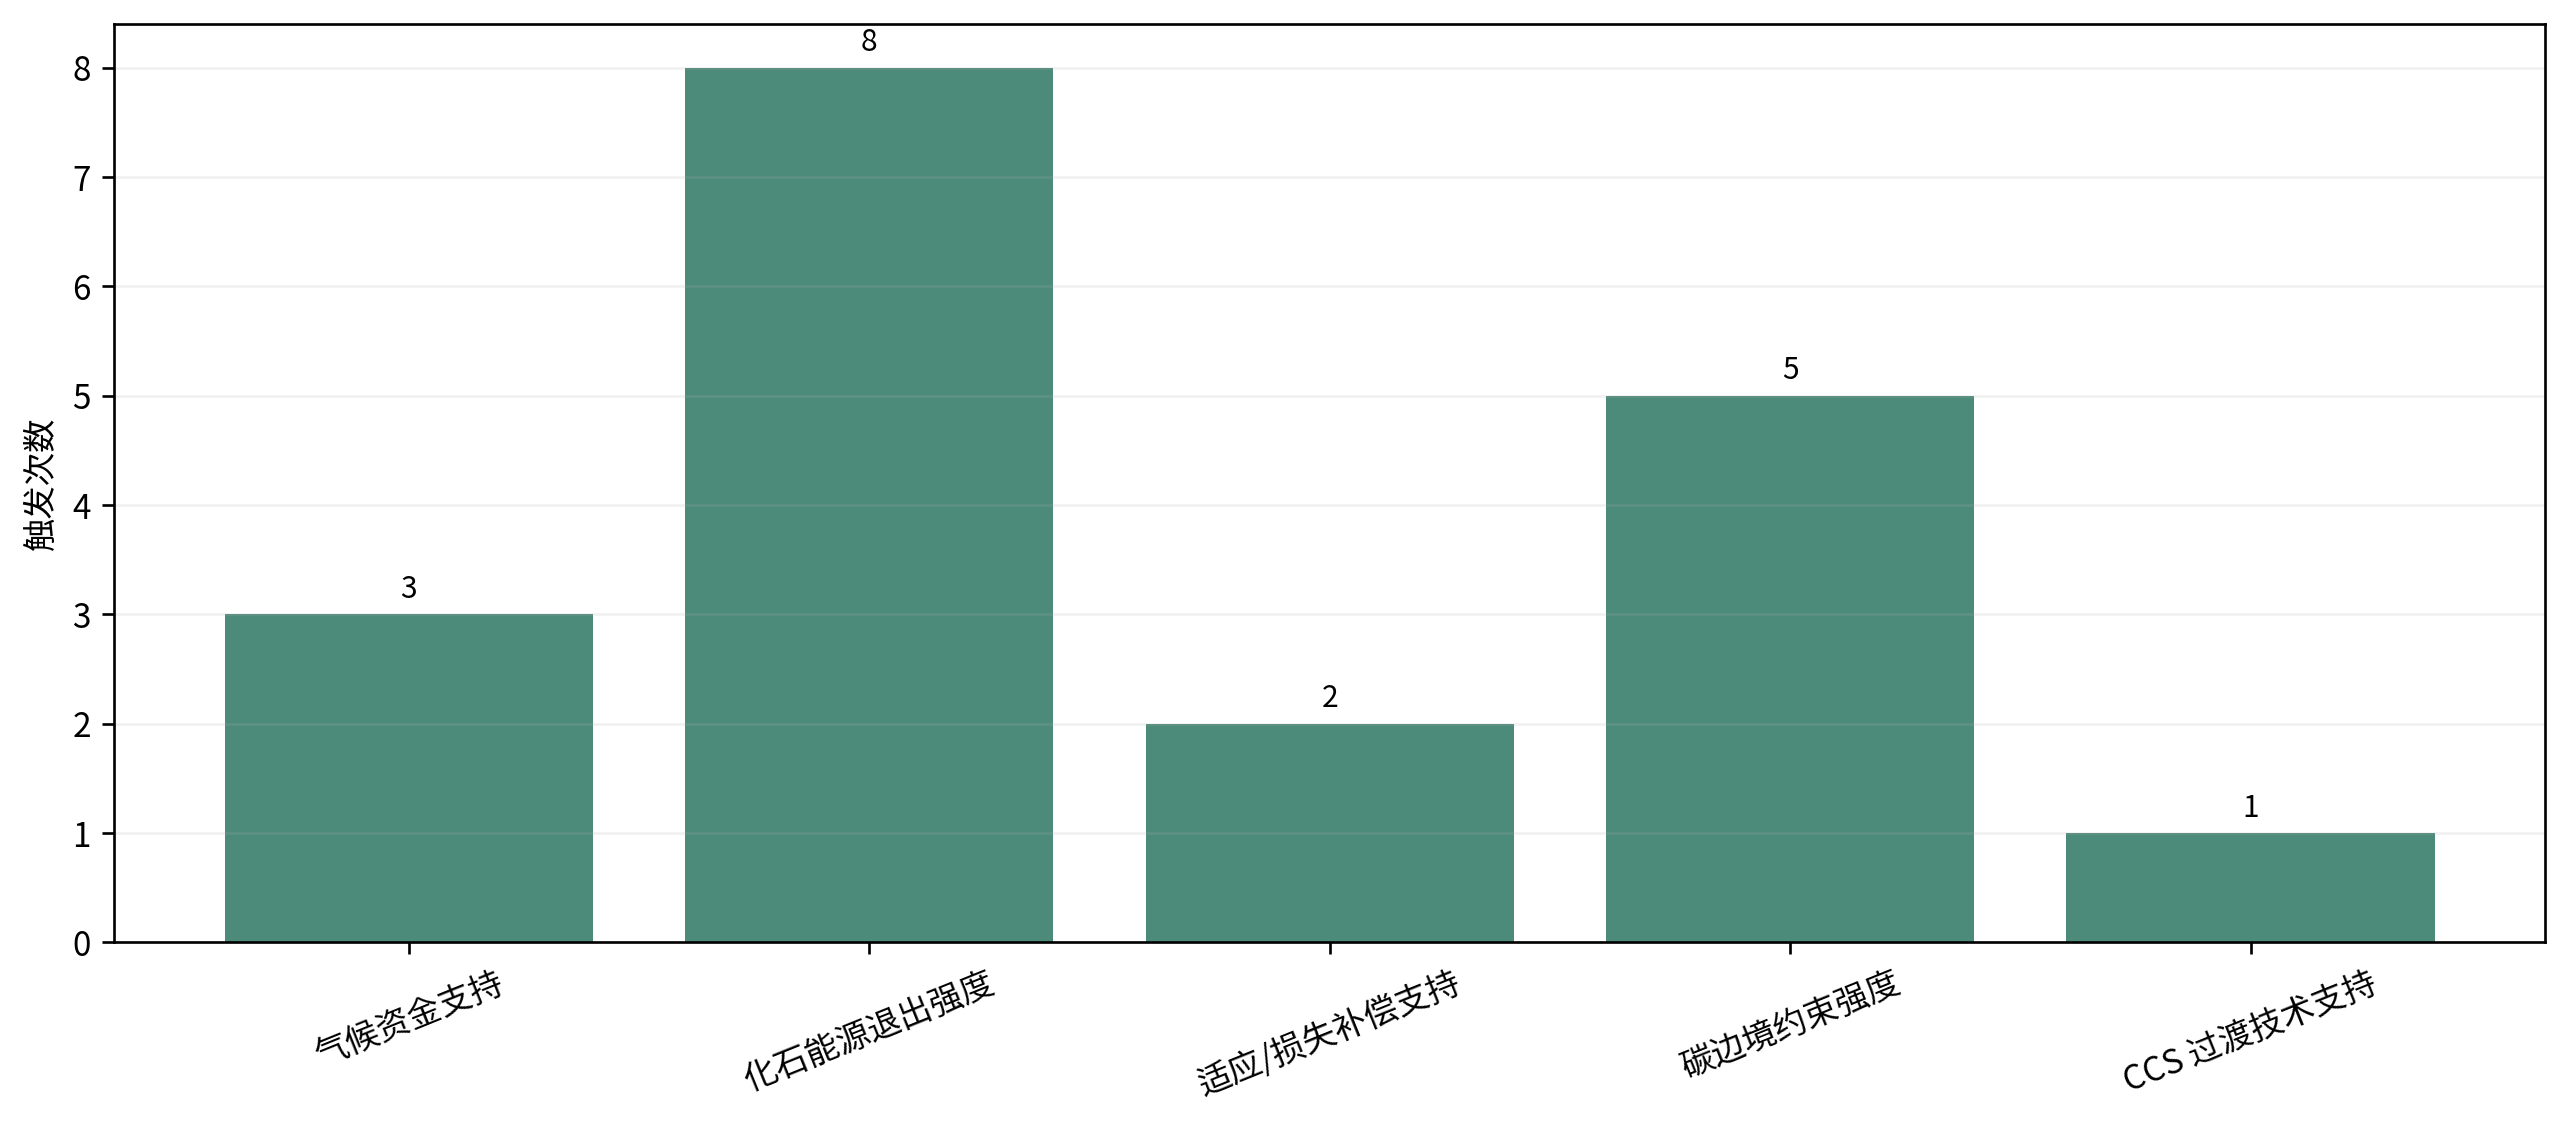
\includegraphics[width=0.9\textwidth]{figures/api_real_constraint_counts.png}
  \caption{真实国家情景实验中的现实约束触发频次}
  \label{fig:constraint}
\end{figure}

可以看到，触发次数最多的约束是 ``化石能源退出强度''（8 次），其次是 ``碳边境约束强度''（5 次）和 ``气候资金支持''（3 次）。这说明：
\begin{itemize}
  \item 对真实国家而言，化石退出时程依然是最敏感的议题；
  \item 贸易型约束会显著增加政策阻力；
  \item 如果资金支持安排不足，即使总体政策方向合理，也很容易破坏共识。
\end{itemize}

这与现实气候谈判中 ``谁来承担转型成本'' 和 ``谁能接受多强约束'' 的核心矛盾高度一致。

\subsection{真实国家样本在两类政策下的变化}
图~\ref{fig:country-compare} 对比了真实国家样本在 E3 和 E4 中的最终得分变化。

\begin{figure}[H]
  \centering
  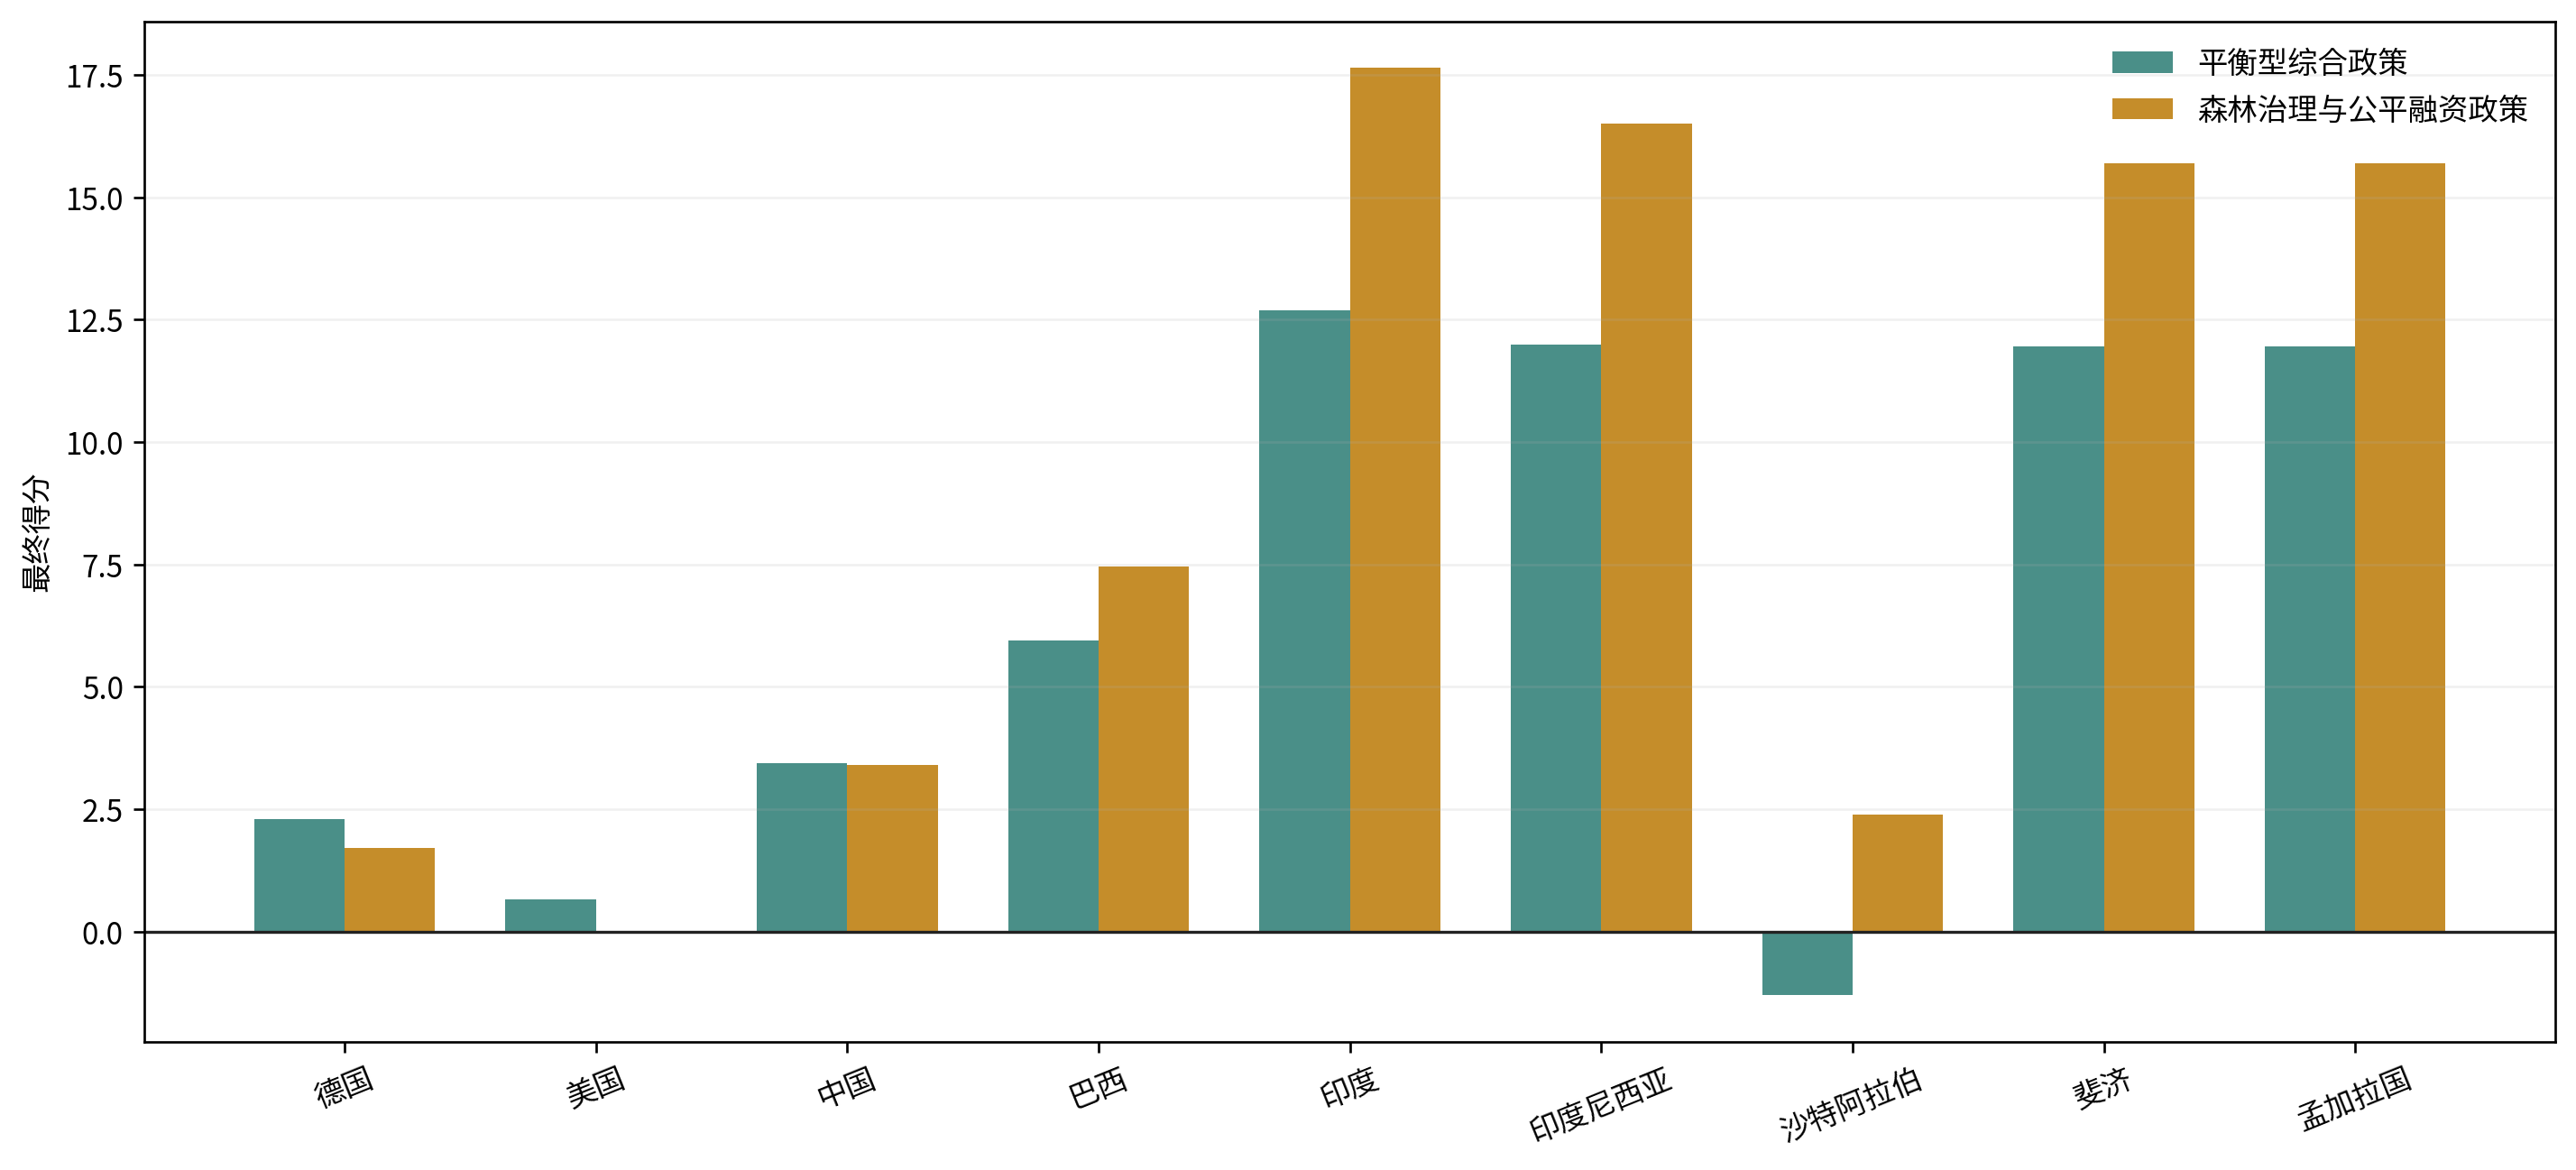
\includegraphics[width=0.97\textwidth]{figures/api_real_position_compare.png}
  \caption{真实国家样本在两类政策下的最终立场得分对比}
  \label{fig:country-compare}
\end{figure}

从图中可以直接观察到：
\begin{itemize}
  \item 巴西、印度、印度尼西亚、斐济和孟加拉国在森林公平型政策下得分均明显提升；
  \item 沙特阿拉伯在平衡型政策下仍为 ``有保留地反对''，但在森林公平型政策下提升为 ``有保留地支持''；
  \item 德国与美国虽然没有转为强支持，但其立场变化说明发达国家对规则约束和责任分担的敏感度仍然存在。
\end{itemize}

因此，森林治理与公平融资不只是改善 ``公平性'' 这一指标，还会改变具体国家的接受边界和联盟结构。

\subsection{约束惩罚对个体立场的影响}
为了更直观地说明约束建模的作用，图~\ref{fig:constraint-penalty} 比较了 E3 中真实国家样本在约束调整前后的得分。

\begin{figure}[H]
  \centering
  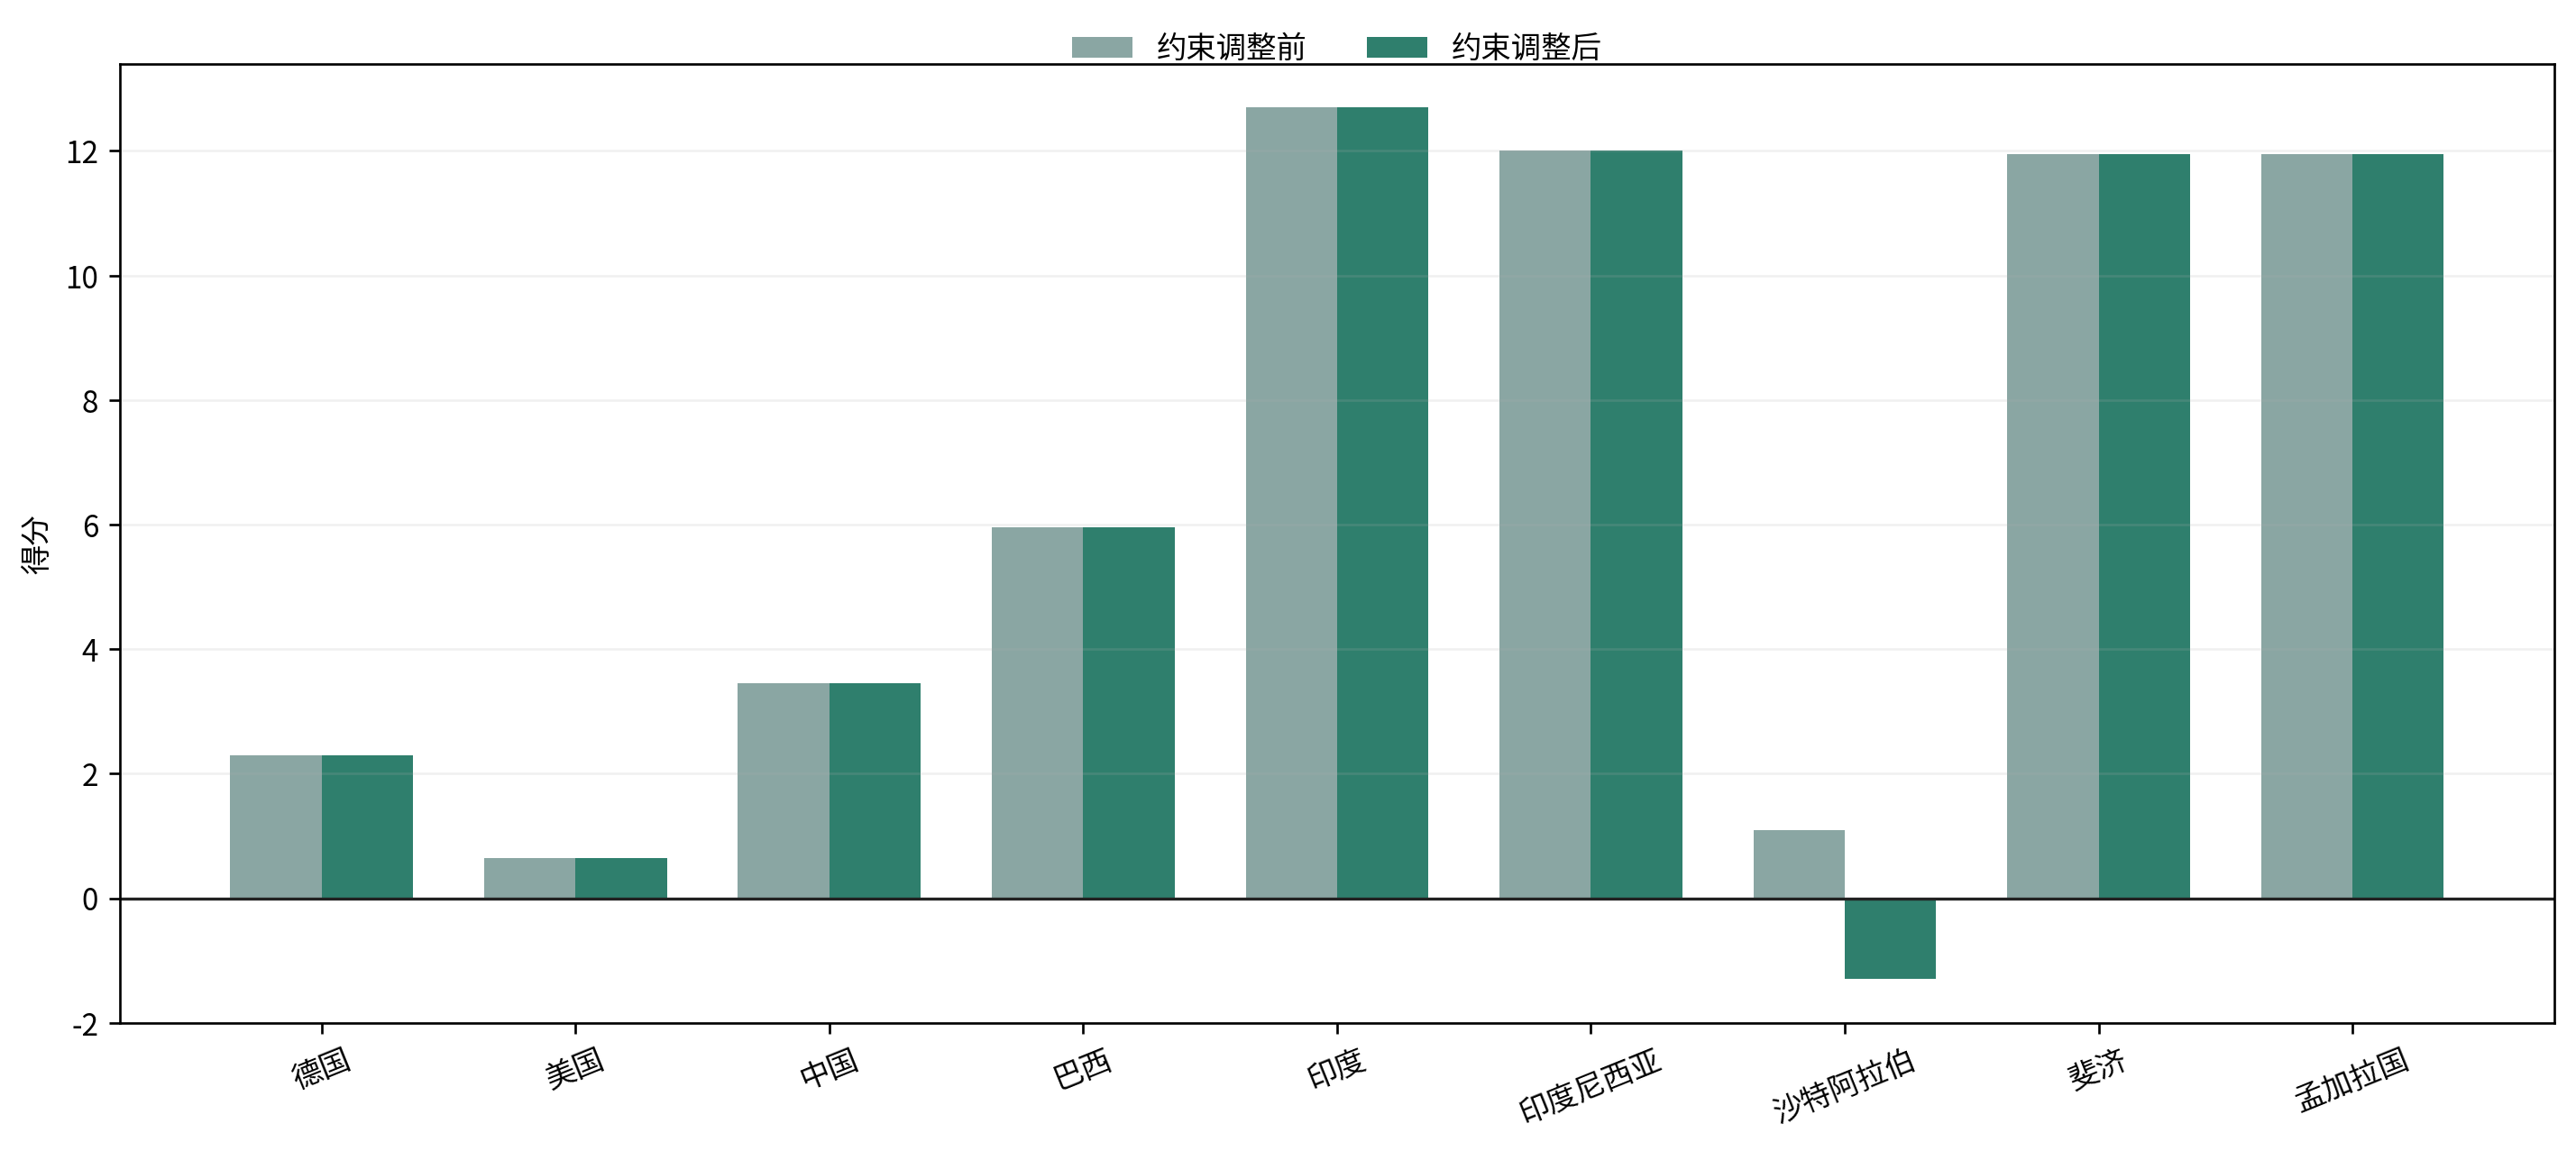
\includegraphics[width=0.97\textwidth]{figures/api_real_constraint_penalty.png}
  \caption{真实国家平衡型政策实验中约束调整前后的角色得分}
  \label{fig:constraint-penalty}
\end{figure}

从图中可以看到，大多数国家在该政策下并未触发足以改变立场类别的硬约束，但 \textbf{沙特阿拉伯} 的变化最为明显：其原始得分为 1.1，经约束惩罚后下降到 -1.3，立场由 ``有保留地支持'' 转为 ``有保留地反对''。这说明真实国家约束并不只是作为说明性注释存在，而是会在关键样本上实质改变协商结果。换言之，约束建模的价值不在于让所有主体都被惩罚，而在于把最重要的现实摩擦点显式暴露出来。

\subsection{模块对比与消融实验}
为了进一步验证系统中不同模块的作用，我们又在实际 API 运行基础上增加了一组方法层面的模块对比实验。图~\ref{fig:ablation} 给出了 5 组对比结果，表~\ref{tab:ablation} 列出了具体数值。

\begin{figure}[H]
  \centering
  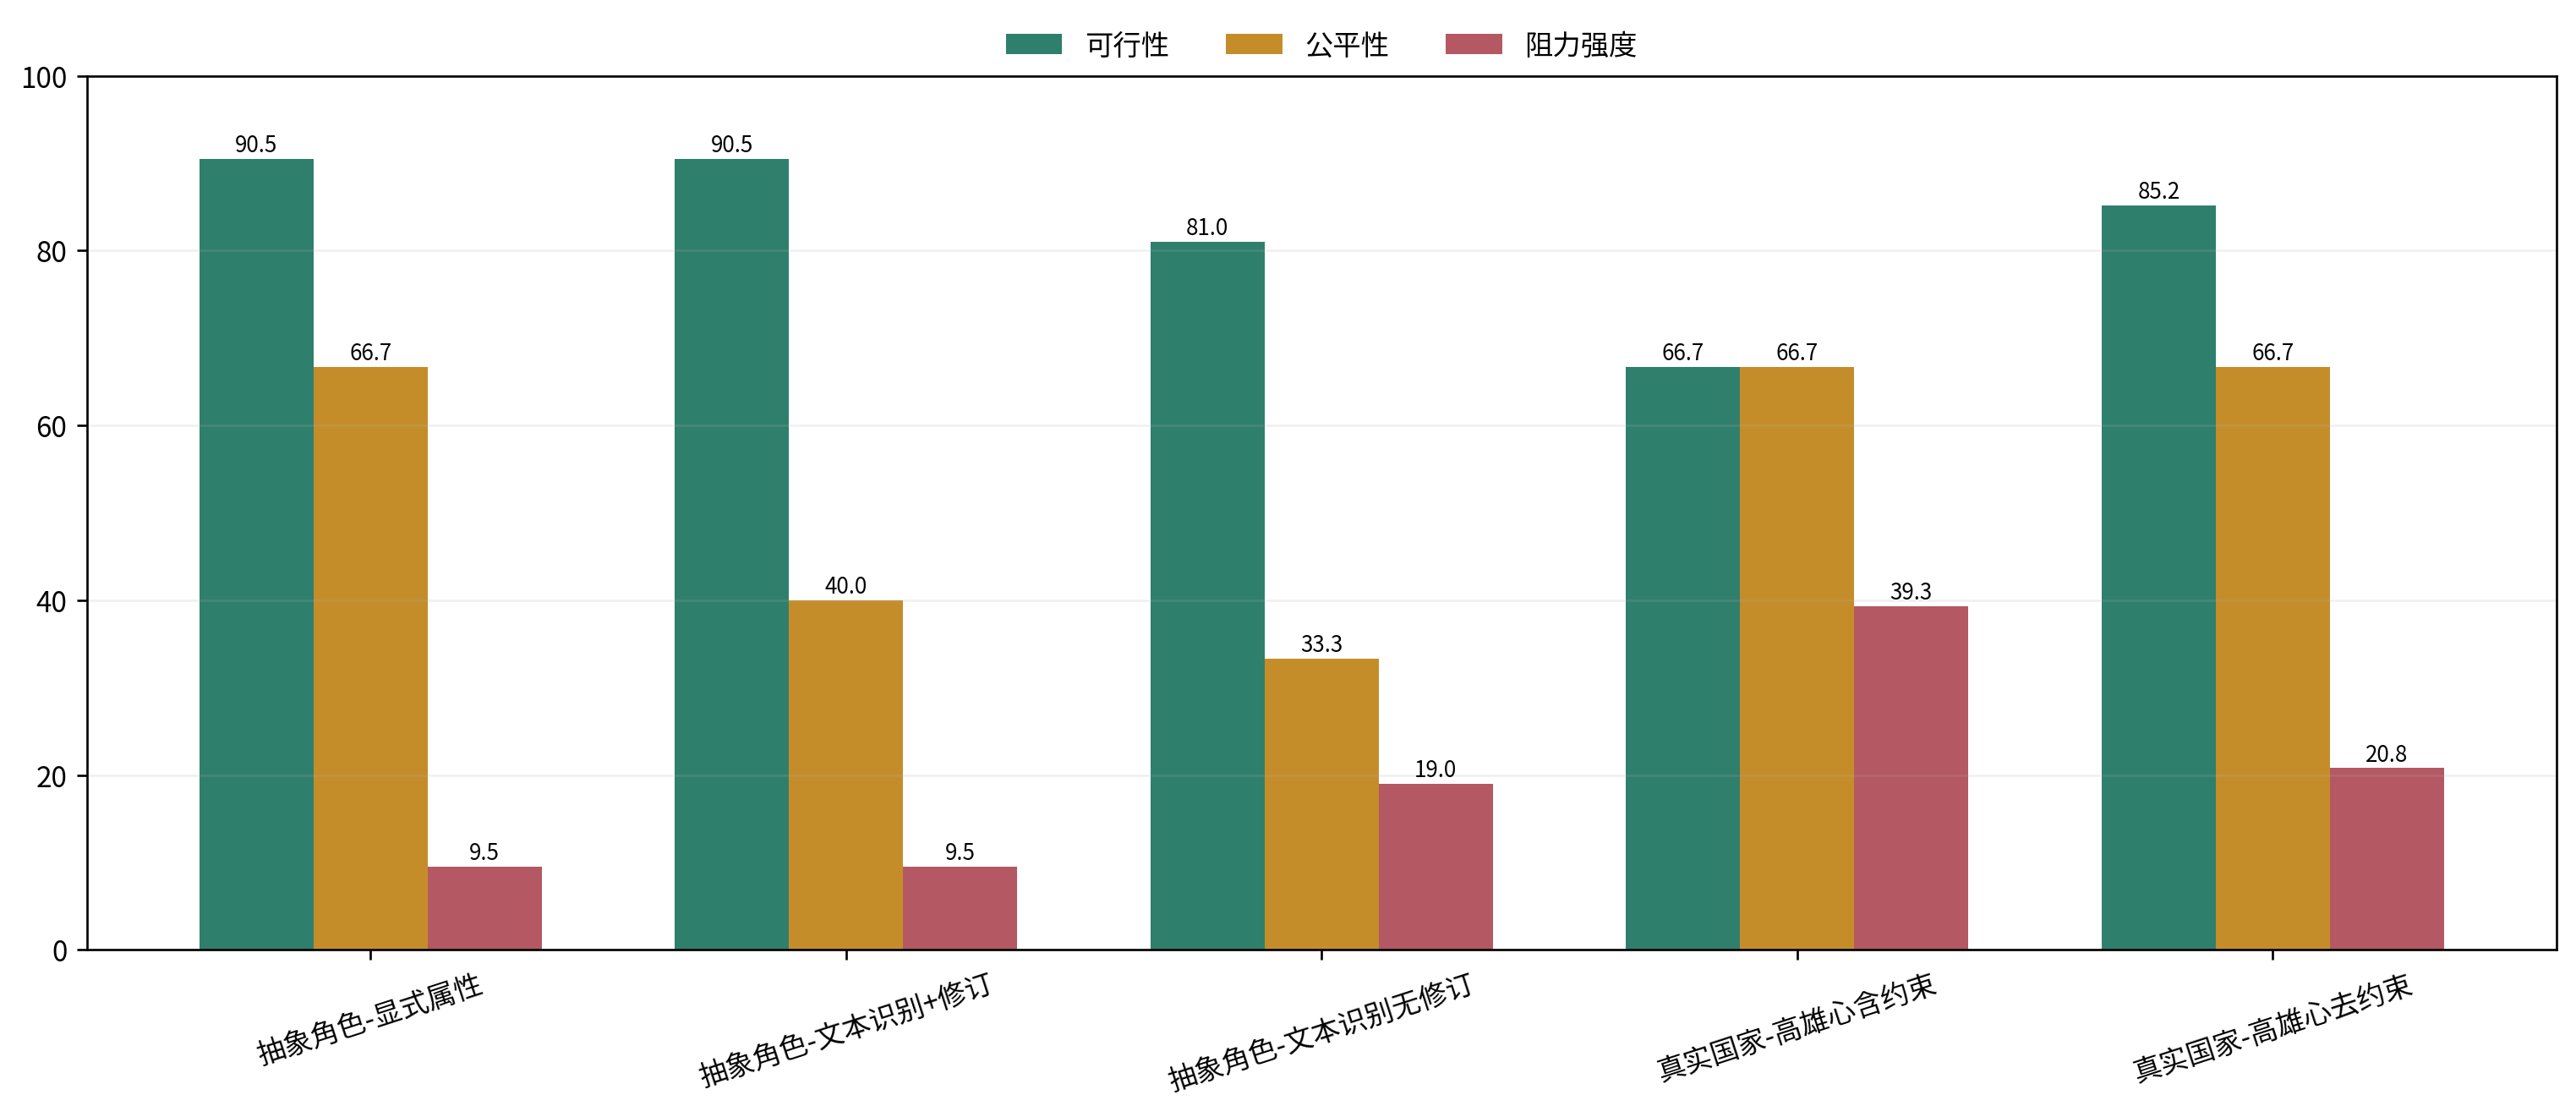
\includegraphics[width=0.98\textwidth]{figures/api_method_ablation_compare.png}
  \caption{方法模块对比实验结果}
  \label{fig:ablation}
\end{figure}

\begin{table}[H]
\centering
\caption{方法模块对比实验结果}
\label{tab:ablation}
\begin{tabular}{lcccc}
\toprule
实验 & 共识水平 & 可行性 & 公平性 & 阻力强度 \\
\midrule
显式属性 & 较强共识 & 90.5 & 66.7 & 9.5 \\
文本识别+修订 & 较强共识 & 90.5 & 40.0 & 9.5 \\
文本识别无修订 & 有限妥协 & 81.0 & 33.3 & 19.0 \\
高雄心含约束 & 有限妥协 & 66.7 & 66.7 & 39.3 \\
高雄心去约束 & 较强共识 & 85.2 & 66.7 & 20.8 \\
\bottomrule
\end{tabular}
\end{table}

这一组对比实验提供了三点关键证据：
\begin{enumerate}
  \item \textbf{显式结构化属性提升的是表达精度，而不只是最终分数。} 在平衡型政策上，``显式属性'' 与 ``文本识别+修订'' 的可行性同为 90.5，但公平性由 40.0 提升到 66.7，说明显式属性输入能更完整地表达政策中的融资、技术、适应与 LULUCF 意图；
  \item \textbf{秘书处修订机制对自动识别场景十分关键。} 当只保留文本自动识别而移除修订环节时，可行性由 90.5 降至 81.0，公平性由 40.0 降至 33.3，阻力则由 9.5 上升到 19.0，说明修订机制确实承担了把初始模糊文本修正为最小可接受方案的作用；
  \item \textbf{现实约束决定了高雄心政策能否维持共识。} 在高雄心政策下，保留约束时可行性只有 66.7，阻力达到 39.3，且共触发 10 次现实约束；一旦去除约束，可行性上升到 85.2、阻力降到 20.8，并重新回到较强共识。这说明真实国家模式中的约束建模是影响结果的核心机制，而不是装饰性模块。
\end{enumerate}

从方法论角度看，这组实验的意义在于：它不仅告诉我们 ``系统能不能跑出结果''，还回答了 ``到底是哪些模块在塑造结果''。这使得整套系统从工程原型进一步接近了一篇方法型技术报告应有的论证方式。

\subsection{DeepSeek V4 Pro 叙事样例观察}
为了展示大模型叙事增强在系统中的实际作用，我们不仅运行了 API 实验，也记录了 DeepSeek V4 Pro 返回的角色发言样例。以 E3 的最终表决为例，系统得到如下风格化表态：
\begin{itemize}
  \item \textbf{德国}：肯定逐步停止无减排措施煤电与森林碳汇方向，但对资金义务和过渡期安排提出规则性要求；
  \item \textbf{美国}：支持对高脆弱国家提供资金与技术，但强调责任分担和统一规则；
  \item \textbf{中国}：强调共同但有区别的责任原则，认可技术转移、适应融资和灵活过渡安排；
  \item \textbf{巴西}：明确支持森林保护与碳汇治理安排，并将其与公平转型联系起来。
\end{itemize}

这些样例说明，叙事增强模块在系统中的作用是清晰且有效的：它能够在不改变规则分数的前提下，把结构化立场转写为更自然的协商表达。为了增强这一部分的可核验性，附录进一步保留了 4 条代表性发言文本，作为系统输出风格的直接证据。

\section{讨论}
综合以上结果，可以得到三点更具解释力的讨论结论。

\subsection{结论一：公平性不是附属条件，而是可行性的核心变量}
无论在抽象角色模式还是真实国家模式中，融资、技术转移、适应支持和过渡安排的存在都会显著抬升政策接受度。尤其在真实国家模式下，如果这些配套条件不足，现实约束会被系统大量触发，从而导致可行性下降、阻力上升。

\subsection{结论二：真实国家模式揭示了抽象角色模式看不见的摩擦}
抽象角色模式的优势是结构清晰、结论稳定、便于教学，但它容易高估政策共识。真实国家模式则会把收入水平、燃料出口、NDC 类型与条件性承诺带来的摩擦带回系统中，因此更适合在报告中展示 ``现实世界为什么更难谈成''。

\subsection{结论三：森林/LULUCF 是值得单列的重要议题}
从本轮实验结果看，森林治理与公平融资结合时，能够显著提升巴西、印度、印度尼西亚等样本的接受度，也帮助高脆弱国家形成更强支持。这说明 LULUCF 维度并非附属性设计，而是推动系统贴近真实政策议题结构的重要组成部分。

\section{局限性、有效性威胁与后续方向}
尽管我们已经完成了一个较完整的课程原型，但仍需诚实说明它的边界：
\begin{itemize}
  \item \textbf{规则驱动边界}：当前可行性、公平性和阻力强度仍来自规则映射，而非计量模型或历史谈判数据训练；
  \item \textbf{角色边界}：抽象角色是研究建模中的典型化对象，不能直接等同于现实世界中某一国家或组织的完整行为；
  \item \textbf{国家样本边界}：真实国家模式已经引入公开数据和 NDC 摘要，但仍属于 ``有来源约束的规则近似''；
  \item \textbf{LLM 边界}：DeepSeek V4 Pro 主要负责叙事增强，而不是让角色独立规划和自由协商。
\end{itemize}

后续最自然的升级方向包括：
\begin{itemize}
  \item 将原版规则引擎升级为真正的多 agent runtime；
  \item 为每个主体增加长期 memory、私下消息通道与自主规划机制；
  \item 引入更完整的联盟网络可视化、私下互动时间线与记忆回放；
  \item 继续扩展真实国家样本的结构化约束与 NDC 条款解析粒度。
\end{itemize}

\section{结论}
本文围绕气候政策多利益相关方博弈沙盘系统展开，在内容组织和证据呈现上做了三项强化：
\begin{enumerate}
  \item 用正式技术报告/论文体结构系统梳理了研究问题、大模型辅助工作流程、系统方法、关键代码模块、展示层设计、实验设计和结果分析；
  \item 将角色设计、数据来源、术语解释与实验可复现性补入附录，覆盖了项目中容易被忽略但对高分评审很重要的内容；
  \item 将正文结果统一建立在本轮实际实验基础之上，以保证全文引用的结论与实验记录一致。
\end{enumerate}

结合实验结果，我们最终得到三条最重要的结论：
\begin{itemize}
  \item 高强度减排和贸易约束若缺乏融资、技术、适应和过渡安排，容易迅速激化冲突；
  \item 真实国家样本模式比抽象角色模式更能揭示政策协商中的现实摩擦；
  \item 森林/LULUCF 与公平融资安排是推动新兴经济体和高脆弱国家形成更高接受度的重要机制。
\end{itemize}

综合来看，本文不仅回答了一个清晰且有意义的气候治理问题，也展示了一种将规则推演、结构化建模与叙事增强结合起来的实现路径。该系统已经具备较完整的方法链路、实验支撑与展示能力，可作为气候政策协商分析与教学展示的有效原型。

\appendix

\section{术语与概念说明}
\begin{itemize}
  \item \textbf{可行性}：最终支持程度的归一化指标，不代表现实世界政策一定能实施，而代表在当前模型中的可接受性。
  \item \textbf{公平性}：对融资、技术转移、适应支持、过渡安排和 LULUCF 支持的综合度量。
  \item \textbf{阻力强度}：综合支持度与约束压力后的阻力指标，值越高表示谈判阻力越大。
  \item \textbf{抽象角色模式}：使用典型利益相关方角色而非真实国家样本进行推演。
  \item \textbf{真实国家样本模式}：使用真实国家指标、NDC 摘要和约束规则生成国家角色。
  \item \textbf{LULUCF}：土地利用、土地利用变化和林业（Land Use, Land-Use Change and Forestry）。
\end{itemize}

\section{抽象角色设计摘要}
\begin{longtable}{>{\raggedright\arraybackslash}p{2.8cm} >{\raggedright\arraybackslash}p{2.3cm} >{\raggedright\arraybackslash}p{5.2cm} >{\raggedright\arraybackslash}p{4cm}}
\caption{抽象角色设计摘要}\label{tab:roles}\\
\toprule
角色 & 阵营 & 角色描述 & 关键诉求 \\
\midrule
\endfirsthead
\toprule
角色 & 阵营 & 角色描述 & 关键诉求 \\
\midrule
\endhead
发达国家联盟 & 高雄心减排方 & 强调更快减排、透明核查和国际规则，希望用更高标准推动全球转型。 & 化石退出、碳边境约束、技术合作 \\
大型新兴经济体 & 发展与转型平衡方 & 强调发展权、能源安全和产业升级，希望在减排与增长之间保留政策空间。 & 融资、技术转移、过渡安排、反对单边约束 \\
最不发达国家集团 & 能力不足但高脆弱方 & 排放责任较低、能力较弱，更关注资金可得性、适应支持和公平转型。 & 融资、适应支持、技术转移 \\
小岛屿与高脆弱国家联盟 & 高脆弱高雄心方 & 强调气候风险紧迫性、损失与损害和 1.5\,$^{\circ}$C 目标。 & 强减排、适应补偿、融资支持 \\
化石能源出口国集团 & 资源与收入维护方 & 关注出口收入、财政稳定与资产搁浅风险，偏好渐进退出和过渡技术。 & 过渡灵活性、CCS、弱化退出与碳边境约束 \\
清洁技术与低碳产业联盟 & 产业升级推动方 & 支持明确的转型信号和技术扩散，希望政策兼顾市场激励与技术合作。 & 技术转移、减排信号、产业投资 \\
多边开发金融机构 & 执行与融资协调方 & 重视政策可实施性、融资撬动和项目落地。 & 融资、技术合作、适应支持、可执行过渡安排 \\
\bottomrule
\end{longtable}

\section{真实国家样本与数据来源摘要}
\begin{longtable}{>{\raggedright\arraybackslash}p{2cm} >{\raggedright\arraybackslash}p{2.5cm} >{\raggedright\arraybackslash}p{4.8cm} >{\raggedright\arraybackslash}p{4.8cm}}
\caption{真实国家样本与建模依据摘要}\label{tab:countries}\\
\toprule
国家 & 样本定位 & 主要建模依据 & 说明 \\
\midrule
\endfirsthead
\toprule
国家 & 样本定位 & 主要建模依据 & 说明 \\
\midrule
\endhead
德国 & 发达经济体样本 & 高收入、高准备度、欧盟共同 NDC、较低燃料出口占比 & 更强调规则约束和减排可信度 \\
美国 & 发达大国样本 & 高收入、较高准备度、最新已提交 NDC 与政治不确定性并存 & 责任分担与规则约束敏感 \\
中国 & 大型新兴经济体样本 & 中高收入、较强产业转型能力、轨迹型承诺 & 重视技术转移、过渡与共同但有区别责任 \\
巴西 & 森林型新兴经济体样本 & 高 LULUCF 相关性、森林治理重要、绝对减排承诺 & 森林议题是关键支撑项 \\
印度 & 高脆弱发展中大国样本 & 强度目标、融资和技术条件性线索、碳汇目标 & 对公平融资与技术支持高度敏感 \\
印度尼西亚 & 煤电转型与群岛国家样本 & FOLU/LULUCF 和能源转型并存、双路径特征明显 & 过渡安排与森林议题同时重要 \\
沙特阿拉伯 & 化石能源出口国样本 & 高资源出口暴露、动态基线型承诺、支持过渡技术 & 对退出时程和边境约束极敏感 \\
斐济 & 小岛屿高脆弱国家样本 & 高脆弱、高适应需求、条件性支持需求明显 & 倾向高雄心减排与补偿机制 \\
孟加拉国 & 高脆弱低收入国家样本 & 高脆弱、低收入、条件性减排明显依赖融资支持 & 适应资金和技术转移是硬约束 \\
\bottomrule
\end{longtable}

\section{数据来源与可靠性摘要}
\begin{table}[H]
\centering
\caption{系统使用的主要数据来源}
\label{tab:sources}
\begin{tabularx}{\textwidth}{>{\raggedright\arraybackslash}p{3cm} >{\raggedright\arraybackslash}p{1.8cm} >{\raggedright\arraybackslash}X >{\raggedright\arraybackslash}p{3.2cm}}
\toprule
来源 & 可靠性 & 用途 & 主要局限 \\
\midrule
UNFCCC NDC Registry & 高 & 作为国家正式承诺文本的一次来源，用于核对提交时间、目标年份和原始承诺内容。 & 多为 PDF，需要进一步结构化抽取 \\
World Bank Open Data & 较高 & 提供 GDP、人均收入、可再生能源占比、燃料出口占比等国家背景指标。 & 不同指标年份可能不完全一致 \\
ND-GAIN Country Index & 中高 & 提供脆弱性与适应准备度比较，用于生成现实约束。 & 属于复合指数，不应被解释为单一因果变量 \\
Climate Watch & 中高 & 提供 NDC 的结构化摘要与辅助浏览入口。 & 属于二次整理平台，不能替代官方文本 \\
\bottomrule
\end{tabularx}
\end{table}

\section{可复现性说明}
本报告正文中引用的结果主要对应以下运行产物：
\begin{itemize}
  \item \texttt{submission\_original/experiments\_api/api\_abstract\_stress\_single.json}
  \item \texttt{submission\_original/experiments\_api/api\_abstract\_balanced\_single.json}
  \item \texttt{submission\_original/experiments\_api/api\_real\_balanced\_single.json}
  \item \texttt{submission\_original/experiments\_api/api\_real\_forest\_single.json}
  \item \texttt{submission\_original/experiments\_api/api\_abstract\_scenario\_batch.json}
  \item \texttt{submission\_original/experiments\_api/api\_real\_scenario\_batch.json}
  \item \texttt{submission\_original/experiments\_api/api\_core\_experiment\_summary.json}
\end{itemize}

图表由以下脚本自动生成：
\begin{itemize}
  \item \texttt{submission\_original/scripts/run\_api\_core\_experiments.py}
  \item \texttt{submission\_original/scripts/generate\_api\_report\_figures.py}
\end{itemize}

若在本地重新运行，应确保：
\begin{itemize}
  \item 已安装 Python 与报告中使用的依赖；
  \item 已配置 \texttt{OPENAI\_API\_KEY}、\texttt{OPENAI\_BASE\_URL}、\texttt{OPENAI\_API\_PATH} 和 \texttt{OPENAI\_MODEL}；
  \item 当前接口仍可通过 OpenAI-compatible 方式访问 \texttt{deepseek-v4-pro}。
\end{itemize}

\section{实际 API 叙事样例附录}
\begin{longtable}{>{\raggedright\arraybackslash}p{1.8cm} >{\raggedright\arraybackslash}p{2.2cm} >{\raggedright\arraybackslash}p{10cm}}
\caption{DeepSeek V4 Pro 实际返回的代表性角色发言样例}\label{tab:llm-samples}\\
\toprule
角色 & 最终状态 & 发言样例 \\
\midrule
\endfirsthead
\toprule
角色 & 最终状态 & 发言样例 \\
\midrule
\endhead
德国 & 有保留地支持 & 我们肯定逐步停止无减排措施煤电和强化森林碳汇的方向，但当前文本对气候资金义务和过渡期灵活性的安排，可能弱化共同责任和公平竞争环境。德方要求方案中保留有约束力的国际规则，否则我们难以支持。 \\
美国 & 有保留地反对 & 我们支持为高脆弱国家提供适应融资和技术转移，但当前方案在气候资金责任分担和规则约束上过于模糊，将压力过度集中在少数发达国家，令人难以接受。要实现减排和公平过渡，需要建立更具约束力的国际机制，确保所有主要经济体按照统一、透明的规则共同行动。 \\
中国 & 有保留地支持 & 我们欢迎文本中为发展中经济体提供灵活过渡安排，并注意到对技术转移、适应融资的重视，这符合共同但有区别的责任原则。希望发达国家能够确保相关支持可落地、可负担，而不附加新的条件，切实帮助发展中国家在森林碳汇、清洁煤电替代等领域实现公正转型。 \\
巴西 & 支持 & 欢迎文本中强化森林保护与碳汇治理的安排，这与巴西作为森林大国的一贯优先方向高度一致。我们认为通过更可落地的技术转移和能力建设，能够帮助发展中国家在保护生态系统、提升碳汇质量的同时推进能源转型，实现共同的气候目标。 \\
\bottomrule
\end{longtable}

\section*{参考资料}
\begin{enumerate}
  \item UN. \textit{Paris Agreement}. 2015.
  \item IPCC. \textit{Climate Change 2023: Synthesis Report}. 2023.
  \item UNFCCC. \textit{NDC Registry}. \url{https://www4.unfccc.int/sites/NDCStaging/Pages/All.aspx}.
  \item World Bank Open Data. \url{https://data.worldbank.org/}.
  \item ND-GAIN Country Index. \url{https://gain.nd.edu/our-work/country-index/}.
  \item Climate Watch. \url{https://www.climatewatchdata.org/ndcs-explore}.
  \item 项目源码与实验文件：\texttt{prototype\_v1/} 与 \texttt{submission\_original/experiments\_api/}。
\end{enumerate}

\end{document}
